% Options for packages loaded elsewhere
\PassOptionsToPackage{unicode}{hyperref}
\PassOptionsToPackage{hyphens}{url}
%
\documentclass[
]{article}
\usepackage{amsmath,amssymb}
\usepackage{lmodern}
\usepackage{iftex}
\ifPDFTeX
  \usepackage[T1]{fontenc}
  \usepackage[utf8]{inputenc}
  \usepackage{textcomp} % provide euro and other symbols
\else % if luatex or xetex
  \usepackage{unicode-math}
  \defaultfontfeatures{Scale=MatchLowercase}
  \defaultfontfeatures[\rmfamily]{Ligatures=TeX,Scale=1}
\fi
% Use upquote if available, for straight quotes in verbatim environments
\IfFileExists{upquote.sty}{\usepackage{upquote}}{}
\IfFileExists{microtype.sty}{% use microtype if available
  \usepackage[]{microtype}
  \UseMicrotypeSet[protrusion]{basicmath} % disable protrusion for tt fonts
}{}
\makeatletter
\@ifundefined{KOMAClassName}{% if non-KOMA class
  \IfFileExists{parskip.sty}{%
    \usepackage{parskip}
  }{% else
    \setlength{\parindent}{0pt}
    \setlength{\parskip}{6pt plus 2pt minus 1pt}}
}{% if KOMA class
  \KOMAoptions{parskip=half}}
\makeatother
\usepackage{xcolor}
\IfFileExists{xurl.sty}{\usepackage{xurl}}{} % add URL line breaks if available
\IfFileExists{bookmark.sty}{\usepackage{bookmark}}{\usepackage{hyperref}}
\hypersetup{
  hidelinks,
  pdfcreator={LaTeX via pandoc}}
\urlstyle{same} % disable monospaced font for URLs
\usepackage{color}
\usepackage{fancyvrb}
\newcommand{\VerbBar}{|}
\newcommand{\VERB}{\Verb[commandchars=\\\{\}]}
\DefineVerbatimEnvironment{Highlighting}{Verbatim}{commandchars=\\\{\}}
% Add ',fontsize=\small' for more characters per line
\newenvironment{Shaded}{}{}
\newcommand{\AlertTok}[1]{\textcolor[rgb]{1.00,0.00,0.00}{\textbf{#1}}}
\newcommand{\AnnotationTok}[1]{\textcolor[rgb]{0.38,0.63,0.69}{\textbf{\textit{#1}}}}
\newcommand{\AttributeTok}[1]{\textcolor[rgb]{0.49,0.56,0.16}{#1}}
\newcommand{\BaseNTok}[1]{\textcolor[rgb]{0.25,0.63,0.44}{#1}}
\newcommand{\BuiltInTok}[1]{#1}
\newcommand{\CharTok}[1]{\textcolor[rgb]{0.25,0.44,0.63}{#1}}
\newcommand{\CommentTok}[1]{\textcolor[rgb]{0.38,0.63,0.69}{\textit{#1}}}
\newcommand{\CommentVarTok}[1]{\textcolor[rgb]{0.38,0.63,0.69}{\textbf{\textit{#1}}}}
\newcommand{\ConstantTok}[1]{\textcolor[rgb]{0.53,0.00,0.00}{#1}}
\newcommand{\ControlFlowTok}[1]{\textcolor[rgb]{0.00,0.44,0.13}{\textbf{#1}}}
\newcommand{\DataTypeTok}[1]{\textcolor[rgb]{0.56,0.13,0.00}{#1}}
\newcommand{\DecValTok}[1]{\textcolor[rgb]{0.25,0.63,0.44}{#1}}
\newcommand{\DocumentationTok}[1]{\textcolor[rgb]{0.73,0.13,0.13}{\textit{#1}}}
\newcommand{\ErrorTok}[1]{\textcolor[rgb]{1.00,0.00,0.00}{\textbf{#1}}}
\newcommand{\ExtensionTok}[1]{#1}
\newcommand{\FloatTok}[1]{\textcolor[rgb]{0.25,0.63,0.44}{#1}}
\newcommand{\FunctionTok}[1]{\textcolor[rgb]{0.02,0.16,0.49}{#1}}
\newcommand{\ImportTok}[1]{#1}
\newcommand{\InformationTok}[1]{\textcolor[rgb]{0.38,0.63,0.69}{\textbf{\textit{#1}}}}
\newcommand{\KeywordTok}[1]{\textcolor[rgb]{0.00,0.44,0.13}{\textbf{#1}}}
\newcommand{\NormalTok}[1]{#1}
\newcommand{\OperatorTok}[1]{\textcolor[rgb]{0.40,0.40,0.40}{#1}}
\newcommand{\OtherTok}[1]{\textcolor[rgb]{0.00,0.44,0.13}{#1}}
\newcommand{\PreprocessorTok}[1]{\textcolor[rgb]{0.74,0.48,0.00}{#1}}
\newcommand{\RegionMarkerTok}[1]{#1}
\newcommand{\SpecialCharTok}[1]{\textcolor[rgb]{0.25,0.44,0.63}{#1}}
\newcommand{\SpecialStringTok}[1]{\textcolor[rgb]{0.73,0.40,0.53}{#1}}
\newcommand{\StringTok}[1]{\textcolor[rgb]{0.25,0.44,0.63}{#1}}
\newcommand{\VariableTok}[1]{\textcolor[rgb]{0.10,0.09,0.49}{#1}}
\newcommand{\VerbatimStringTok}[1]{\textcolor[rgb]{0.25,0.44,0.63}{#1}}
\newcommand{\WarningTok}[1]{\textcolor[rgb]{0.38,0.63,0.69}{\textbf{\textit{#1}}}}
\usepackage{longtable,booktabs,array}
\usepackage{calc} % for calculating minipage widths
% Correct order of tables after \paragraph or \subparagraph
\usepackage{etoolbox}
\makeatletter
\patchcmd\longtable{\par}{\if@noskipsec\mbox{}\fi\par}{}{}
\makeatother
% Allow footnotes in longtable head/foot
\IfFileExists{footnotehyper.sty}{\usepackage{footnotehyper}}{\usepackage{footnote}}
\makesavenoteenv{longtable}
\usepackage{graphicx}
\makeatletter
\def\maxwidth{\ifdim\Gin@nat@width>\linewidth\linewidth\else\Gin@nat@width\fi}
\def\maxheight{\ifdim\Gin@nat@height>\textheight\textheight\else\Gin@nat@height\fi}
\makeatother
% Scale images if necessary, so that they will not overflow the page
% margins by default, and it is still possible to overwrite the defaults
% using explicit options in \includegraphics[width, height, ...]{}
\setkeys{Gin}{width=\maxwidth,height=\maxheight,keepaspectratio}
% Set default figure placement to htbp
\makeatletter
\def\fps@figure{htbp}
\makeatother
\setlength{\emergencystretch}{3em} % prevent overfull lines
\providecommand{\tightlist}{%
  \setlength{\itemsep}{0pt}\setlength{\parskip}{0pt}}
\setcounter{secnumdepth}{-\maxdimen} % remove section numbering
\ifLuaTeX
  \usepackage{selnolig}  % disable illegal ligatures
\fi

\author{}
\date{}

\begin{document}

\hypertarget{khung-sux1b0ux1eddn}{%
\section{Khung sườn}\label{khung-sux1b0ux1eddn}}

Khung sườn khóa luận kết thúc 6 năm luyện ngục của nvmnghia.

Độ dài yêu cầu: 40-50 trang.

\begin{center}\rule{0.5\linewidth}{0.5pt}\end{center}

\hypertarget{buxeca-cuxe1c-mux1ee5c-liuxean-quan}{%
\subsection{0. Bìa \& các mục liên
quan}\label{buxeca-cuxe1c-mux1ee5c-liuxean-quan}}

\begin{itemize}
\item
  Bìa
\item
  Phụ bìa
\item
  Cam đoan không sao chép
\item
  Phê chuẩn của giảng viên hướng dẫn
\item
  Lời cảm ơn
\item
  Tóm tắt

  Nhờ Internet, truyền hình và điện ảnh, văn hóa truyện tranh đã trở nên
  phổ biến toàn cầu, nhất là trong giới trẻ. Nhu cầu tiêu thụ truyện
  tranh tăng cao thúc đẩy sự phát triển của các trang web truyện tranh
  với ưu điểm là thuận tiện, tốc độ cập nhật truyện nhanh. Tuy nhiên,
  nguồn truyện tranh của những trang web này có chất lượng không cao.
  Một bộ phận người đọc kĩ tính chọn đọc và lưu trữ những tệp truyện
  được số hóa chất lượng cao, thường ở dạng tệp nén đuôi \texttt{cbr} và
  \texttt{cbz}. Xuất phát từ nhu cầu này, tôi muốn viết ứng dụng
  \emph{yacv} có thể đọc các tệp truyện nén trên điện thoại Android.
  Khóa luận sẽ trình bày một số nền tảng của yacv như Android và Kotlin;
  sau đó là các ca sử dụng chính cùng với thiết kế và cài đặt của ứng
  dụng.

  Từ khóa: Android, coroutine, zip, comic
\item
  Mục lục
\item
  Danh sách bảng
\item
  Danh sách hình
\item
  Danh sách kí hiệu, chữ viết tắt

  \begin{itemize}
    \item
    MVC
  \item
    MVP
  \item
    MVVM
  \item
    RDBMS
  \item
    ORM
  \item
    SC
  \end{itemize}
\end{itemize}

\begin{center}\rule{0.5\linewidth}{0.5pt}\end{center}

\hypertarget{chux1b0ux1a1ng-1-giux1edbi-thiux1ec7u}{%
\subsection{\texorpdfstring{1. Chương 1: Giới thiệu
}{1. Chương 1: Giới thiệu }}\label{chux1b0ux1a1ng-1-giux1edbi-thiux1ec7u}}

\hypertarget{ux111ux1eb7t-vux1ea5n-ux111ux1ec1}{%
\subsubsection{\texorpdfstring{1.1. Đặt vấn đề
}{1.1. Đặt vấn đề }}\label{ux111ux1eb7t-vux1ea5n-ux111ux1ec1}}

Tại Đông Á và Đông Nam Á, văn hóa truyện tranh gốc Á, nhất là truyện
tranh Nhật (manga), được đón nhận khá tích cực, đặc biệt trong giới trẻ.
Thế hệ những người dưới 40 tuổi hiện nay được tiếp xúc với truyện tranh
từ sớm, thông qua những cuốn truyện truyền tay và phim hoạt hình dựa
trên truyện tranh, và tiếp tục đọc dù đã qua tuổi thiếu niên. Một số tác
phẩm manga còn có lượng người đọc lớn trên toàn cầu như Doraemon, One
Piece. Ở bên kia bán cầu, với sự thành công của vũ trụ điện ảnh Marvel
và DC, truyện tranh phương Tây (comic) cũng được hồi sinh phần nào sau
một thập kỷ thiếu sáng tạo và suy giảm doanh số sách in. Các bộ truyện
siêu anh hùng, vốn trước đây chỉ phổ biến ở Hoa Kỳ, nay đang trên đường
trở thành một phần của văn hóa đại chúng như vị thế của manga. Có thể
nói, văn hóa truyện tranh nói chung đang ở thời kì phát triển mạnh, xét
theo tiêu chí về độ phổ biến và thái độ đón nhận của xã hội.

Hiện nay, hầu hết mọi người đọc truyện qua các trang web tổng hợp truyện
tranh. Những trang web này có hai ưu điểm chính:

\begin{itemize}
\item
  Số lượng: Mỗi trang cung cấp ít nhất hàng nghìn đầu truyện.
\item
  Tốc độ: Tốc độ ra truyện rất nhanh. Với các bộ truyện nổi tiếng,
  thường chỉ trong vòng một vài giờ sau khi ra mắt, chương mới đã xuất
  hiện.
\end{itemize}

Tuy vậy, nhược điểm chính của những trang web này là chất lượng ảnh của
truyện. Để giảm thời gian tải và tránh tốn băng thông, hình ảnh của
truyện thường được nén khá nhiều, gây vỡ hình, mờ nhòe. Một bộ phận
người đọc, hoặc kĩ tính, hoặc muốn sưu tầm truyện, thường chọn đọc những
tệp truyện chất lượng cao, thường có đuôi CBZ hoặc CBR. Bản chất tệp
truyện này là các tệp nén zip bình thường, bên trong có các tệp ảnh
thông dụng như JPG, PNG. Tuy nhiên, do được tải hẳn về máy rồi mới đọc,
những tệp truyện này không bị giới hạn về băng thông hay thời gian, do
đó hình ảnh trong tệp có thể có chất lượng rất cao.

Trong khóa luận này, tôi viết một ứng dụng Android nhằm phục vụ số ít
người dùng có nhu cầu đọc truyện tranh chất lượng cao đã giới thiệu ở
trên. Tên của ứng dụng là ``yacv'', viết tắt của cụm từ tiếng Anh ``Yet
Another Comic Viewer'', tạm dịch là ``Lại một ứng dụng xem truyện tranh
nữa''. Hai tính năng chính duy nhất của ứng dụng là đọc và quản lí cơ
bản (tìm kiếm, xóa) tệp truyện tranh có sẵn trên điện thoại.

Cần chú ý rằng ứng dụng yacv chỉ bao gồm các tính năng liên quan đến đọc
truyện ngoại tuyến, đọc các tệp truyện có sẵn trên điện thoại người
dùng. Ứng dụng không phải là ứng dụng khách cho các trang đọc truyện
hiện có, hay có máy chủ tập trung riêng để cung cấp truyện.

\hypertarget{ux1ee9ng-dux1ee5ng-tux1b0ux1a1ng-tux1ef1}{%
\subsubsection{\texorpdfstring{1.2. Ứng dụng tương tự
}{1.2. Ứng dụng tương tự }}\label{ux1ee9ng-dux1ee5ng-tux1b0ux1a1ng-tux1ef1}}

Hiện có nhiều ứng dụng đọc truyện tranh ngoại tuyến như yacv trên chợ
ứng dụng Google Play. Hai ứng dụng phổ biến nhất trong số này là
\href{https://play.google.com/store/apps/details?id=com.viewer.comicscreen\&hl=en\&gl=US}{ComicScreen}
và
\href{https://play.google.com/store/apps/details?id=com.aerilys.acr.android\&hl=en\&gl=US}{Astonishing
Comic Reader}. ComicScreen là ứng dụng có nhiều người dùng hơn. Các tính
năng của ComicScreen giống với các tính năng của yacv, tuy nhiên
ComicScreen có thêm nhiều chức năng phụ, đáng kể nhất là khả năng đọc từ
mạng FTP/SMB và khả năng sửa ảnh trong file. Astonishing Comic Reader
cũng có chức năng tương tự yacv, không hơn, tuy nhiên giao diện khá trau
chuốt. Cả hai đều miễn phí và có quảng cáo, được cập nhật có thể nói là
thường xuyên.

Một ngoại lệ đáng kể ở đây là ứng dụng mã nguồn mở
\href{https://github.com/tachiyomiorg/tachiyomi}{Tachiyomi}. Ứng dụng
này có hệ thống phần mở rộng, cho phép đọc truyện ở các trang web truyện
tranh. Khi web truyện tranh thay đổi, hoặc hỗ trợ thêm trang mới, chỉ
cần tải về phần mở rộng tương ứng ở dạng ứng dụng APK. Tính năng này
cùng mô hình mã nguồn mở khiến Tachiyomi mạnh hơn, cập nhật nhanh hơn
toàn bộ các ứng dụng đã có và sẽ có. Tuy nhiên, Tachiyomi lại không thể
được đưa lên Play Store, vì chính tính năng phần mở rộng đã
\href{https://github.com/tachiyomiorg/tachiyomi/issues/1745}{vi phạm
chính sách} của Play Store.

Một điểm khác biệt quan trọng của yacv với các ứng dụng có sẵn là việc
hỗ trợ metadata của tệp truyện tranh, do các ứng dụng có sẵn trên Play
Store đa số bỏ qua thông tin này trong tệp truyện. Một trong số rất ít
những ứng dụng hỗ trợ tính năng này là
\href{https://play.google.com/store/apps/details?id=br.com.kurotoshiro.leitor_manga\&hl=en\&gl=US}{Kuro
Reader}, tuy nhiên đây là một tính năng trả phí.

\hypertarget{kux1ebft-quux1ea3-ux111ux1ea1t-ux111ux1b0ux1ee3c}{%
\subsubsection{\texorpdfstring{1.3. Kết quả đạt được
}{1.3. Kết quả đạt được }}\label{kux1ebft-quux1ea3-ux111ux1ea1t-ux111ux1b0ux1ee3c}}

Ứng dụng có các tính năng đủ dùng theo mục đích đã đề ra:

\begin{itemize}
\item
  Đọc file truyện CBZ
\item
  Tìm kiếm truyện theo metadata
\end{itemize}

Tính năng đọc tệp truyện CBR hiện mới chỉ được cài đặt một phần, do khó
khăn trong việc tích hợp thư viện đọc định dạng này.

\hypertarget{cux1ea5u-truxfac-khuxf3a-luux1eadn}{%
\subsubsection{\texorpdfstring{1.4. Cấu trúc khóa luận
}{1.4. Cấu trúc khóa luận }}\label{cux1ea5u-truxfac-khuxf3a-luux1eadn}}

Các phần còn lại của khóa luận có cấu trúc như sau:

\begin{itemize}
\item
  \protect\hyperlink{P2-fundamental}{Chương 2 - Kiến thức nền tảng}:
  Giới thiệu sơ lược về ba nền tảng của ứng dụng, gồm hệ điều hành
  Android, ngôn ngữ lập trình Kotlin, và mẫu thiết kế MVVM; định dạng
  tệp nén ZIP cũng được giới thiệu vì liên quan trực tiếp đến ứng dụng.
\item
  \protect\hyperlink{P3-requirements}{Chương 3 - Phân tích yêu cầu}:
  Phân tích nhu cầu và ca sử dụng để có đặc tả yêu cầu.
\item
  \protect\hyperlink{P4-design}{Chương 4 - Thiết kế}: Thiết kế ứng dụng,
  gồm thiết kế cơ sở dữ liệu, giao diện, logic nghiệp vụ.
\item
  \protect\hyperlink{P5-implementation}{Chương 5 - Lập trình \& Kiểm
  thử}: Một số cài đặt và ca kiểm thử trong ứng dụng sẽ được nêu một
  cách có chọn lọc.
\item
  \protect\hyperlink{P6-comclusion}{Chương 6 - Kết luận}: Kết thúc khóa
  luận.
\end{itemize}

\begin{center}\rule{0.5\linewidth}{0.5pt}\end{center}

\hypertarget{chux1b0ux1a1ng-2-kiux1ebfn-thux1ee9c-nux1ec1n-tux1ea3ng}{%
\subsection{\texorpdfstring{2. Chương 2: Kiến thức nền tảng
}{2. Chương 2: Kiến thức nền tảng }}\label{chux1b0ux1a1ng-2-kiux1ebfn-thux1ee9c-nux1ec1n-tux1ea3ng}}

Chương này giới thiệu sơ qua về các nền tảng trong quá trình xây dựng
ứng dụng.

\begin{itemize}
\item
  Hai nền tảng đầu tiên liên quan đến nhau, là tiền đề cho toàn bộ ứng
  dụng sẽ được giới thiệu trước, gồm hệ điều hành Android và ngôn ngữ
  lập trình Kotlin.
\item
  Tiếp theo, lựa chọn về kiến trúc tổng quan, liên quan đến giao diện
  của ứng dụng được trình bày.
\item
  Sau đó, cơ sở dữ liệu một số phần mở rộng của nó dùng trong ứng dụng
  sẽ được nhắc qua.
\item
  Cuối cùng là thông tin về CBZ - định dạng tệp tin mà ứng dụng đọc.
\end{itemize}

\hypertarget{hux1ec7-ux111iux1ec1u-huxe0nh-android}{%
\subsubsection{\texorpdfstring{2.1. Hệ điều hành Android
}{2.1. Hệ điều hành Android }}\label{hux1ec7-ux111iux1ec1u-huxe0nh-android}}

Android là một hệ điều hành di động do Google phát triển. Android dùng
nhân Linux và được thiết kế cho màn hình cảm ứng. Cùng với iOS của
Apple, Android trở thành một phần không thể thiếu của cuộc cách mạng di
động bắt đầu vào cuối những năm 2000.

Google mua lại phiên bản Android đầu của công ty khởi nghiệp cùng tên
vào năm 2005, và phát triển nó từ đó. Ngoài Google, Android còn nhận
đóng góp lớn từ cộng đồng, do có mã nguồn mở (phần lớn dùng giấy phép
Apache); tên chính thức của dự án là Android Open Source Project. Dù
vậy, mọi thiết bị Android thương mại đều có ứng dụng độc quyền. Ví dụ
đáng kể là bộ Google Mobile Services, chứa những ứng dụng thiết yếu như
trình duyệt Chrome hay chợ Play Store. Về mặt này, Android khá giống
Chrome: thành phần cốt lõi kĩ thuật được phát triển theo mô hình mã
nguồn mở (AOSP và Chromium), còn thành phần liên quan đến trải nghiệm
người dùng được phát triển riêng.

\begin{figure}
\centering
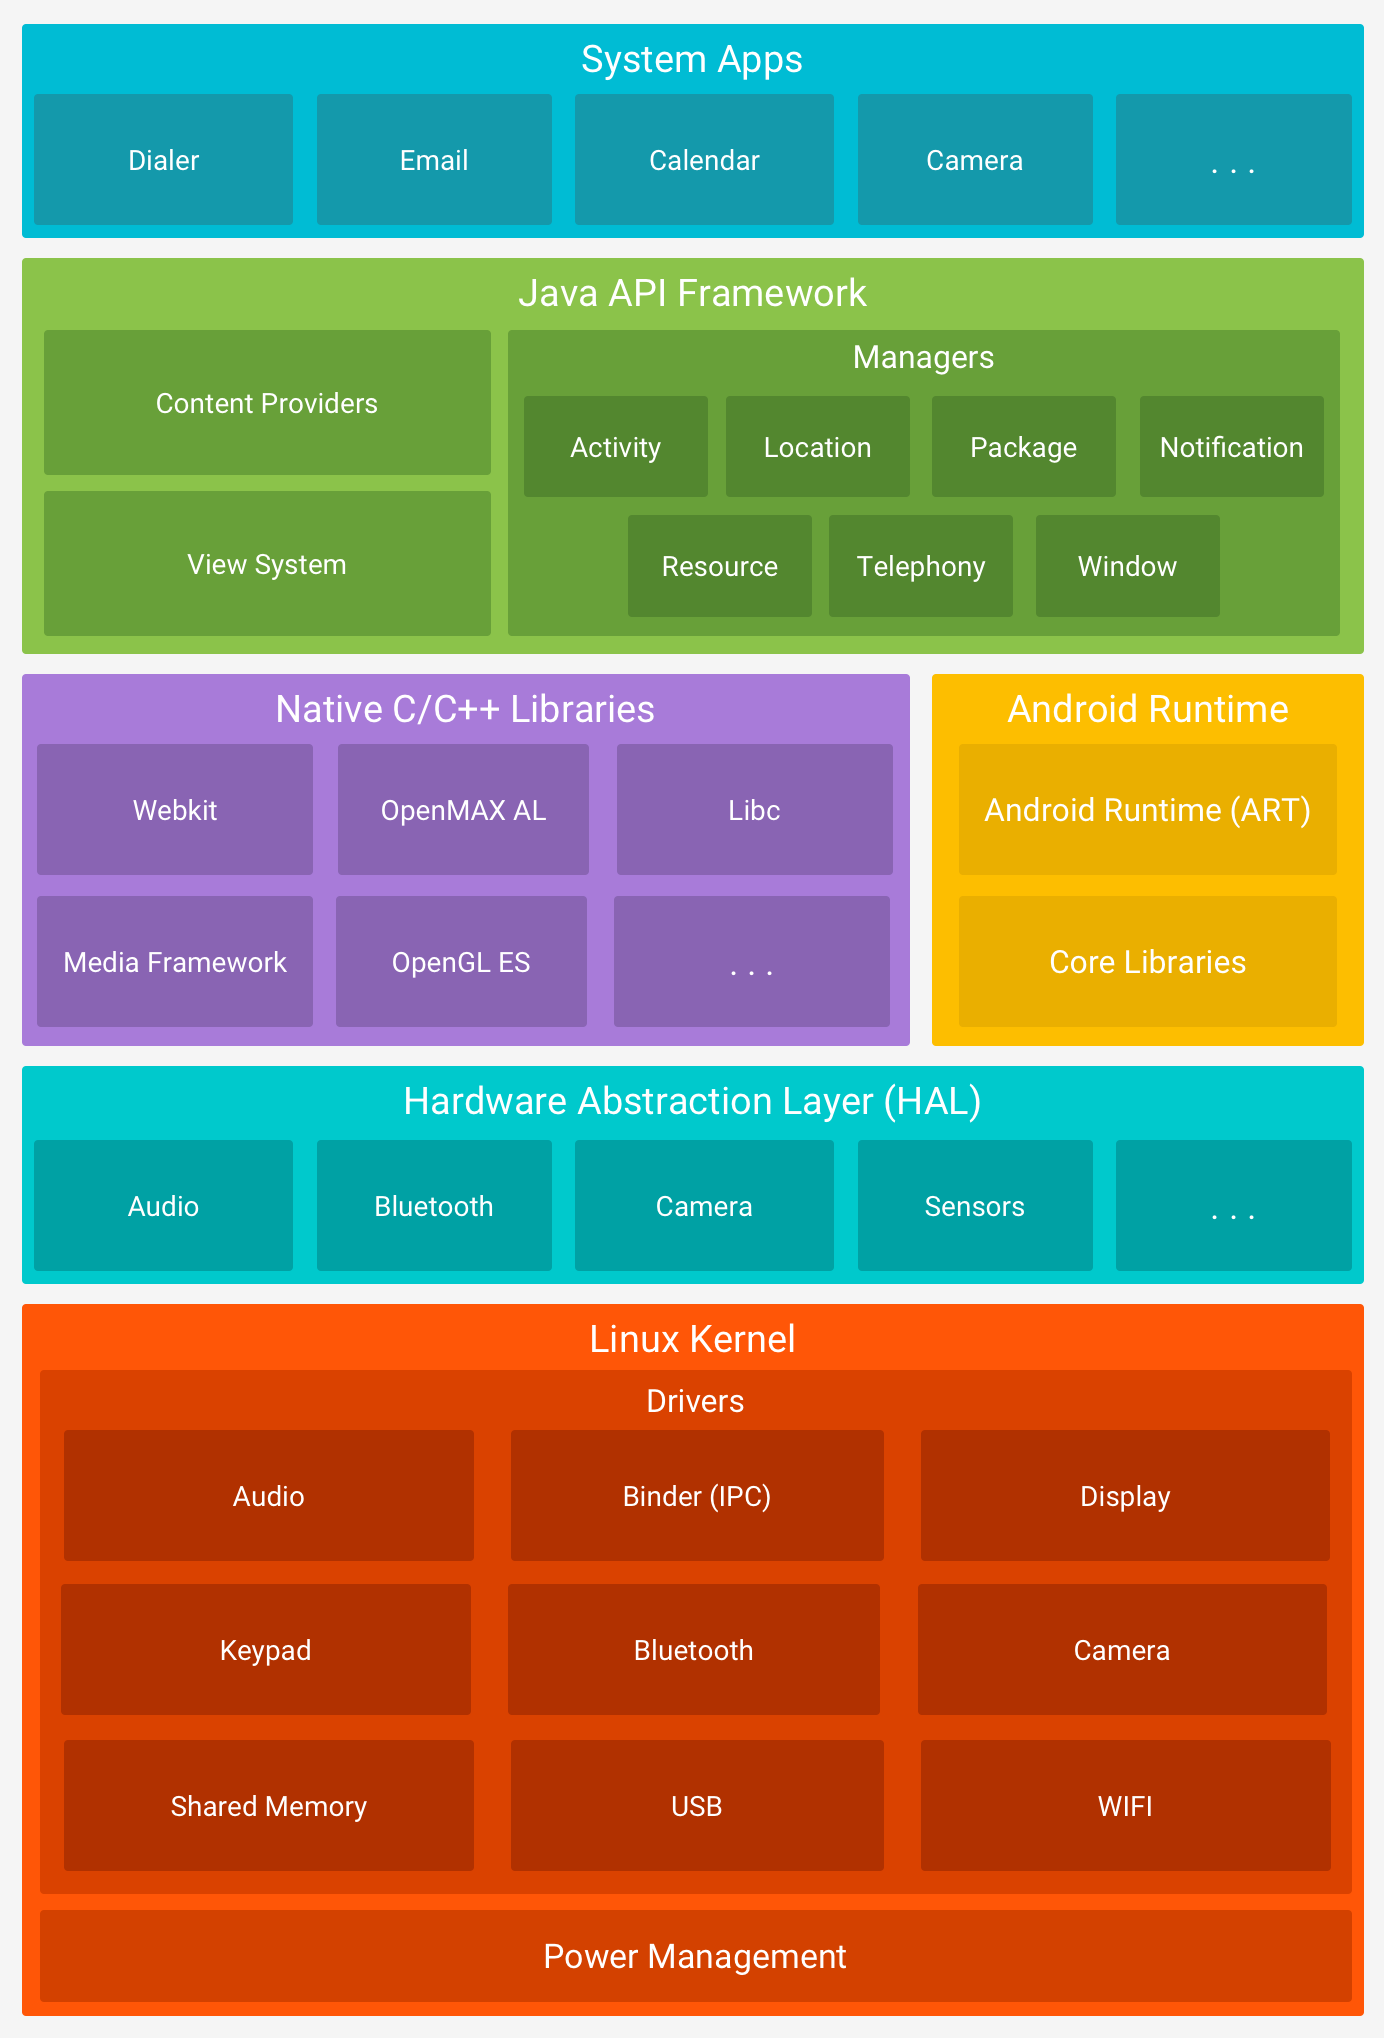
\includegraphics{../images/android-stack_2x.png}
\caption{Android software stack}
\end{figure}

Hình 1: Các phân lớp của hệ điều hành Android

Android được phân lớp như sau:

\begin{itemize}
\item
  Nhân Linux (Linux Kernel):

  Android dùng nhánh hỗ trợ dài hạn (LTS) của Linux. Khác kiểu phát
  triển distro trên máy tính (chủ yếu thay đổi ở ngoài nhân), Google sửa
  nhân khá nhiều trước khi tích hợp.
\item
  Lớp phần cứng trừu tượng (Hardware Abstraction Layer):

  Tầng này đưa ra giao diện chung cho mỗi kiểu phần cứng (máy ảnh,
  loa,\ldots), giúp các tầng trên có thể dùng phần cứng mà không quan
  tâm đến chi tiết riêng.
\item
  Android Runtime (ART):

  Ứng dụng Java cần thêm một ứng dụng để chuyển bytecode thành mã máy.
  Trên desktop, đó là các máy ảo Java (JVM). Trên Android, Android
  Runtime nhận nhiệm vụ này. Hai máy ảo này khác nhau ở chỗ ART
  \emph{biên dịch} bytecode thành mã máy (trước khi chạy - AOT), còn JVM
  \emph{thông dịch} bytecode thành mã máy (trong khi chạy).
\item
  Thư viện C/C++:

  Tầng này phục vụ một số ứng dụng dùng NDK (từ Java gọi C) như trò chơi
  điện tử.
\item
  Khung phát triển ứng dụng (Java API Framework):

  Mọi ứng dụng Java được viết nhờ sử dụng các thành phần của tầng này
  thông qua API Java. Tầng này cung cấp toàn bộ tính năng của Android
  cho lập trình viên, bao gồm các yếu tố cơ bản như giao diện (View
  System), truy xuất,\ldots{}

  Lập trình viên có thể truy cập vào lớp này tương đương với ứng dụng hệ
  thống. Đây được coi là một cam kết tránh độc quyền công nghệ, tức đa
  số ứng dụng hệ thống không có khả năng đặc biệt hơn ứng dụng bên thứ
  ba tương tự.
\item
  Ứng dụng hệ thống (System Apps)

  Android đi kèm với một số ứng dụng hệ thống như ứng dụng SMS, trình
  duyệt, lịch,\ldots{} Google cho phép thay thế đa số các ứng dụng này
  với ứng dụng bên thứ ba, tuy nhiên có những ngoại lệ như ứng dụng Cài
  đặt (Settings).
\end{itemize}

Gần như mọi ứng dụng Android cơ bản đều dùng View System trong tầng
Khung phát triển để viết giao diện, và yacv không là ngoại lệ. yacv còn
sử dụng thành phần Content Provider, cụ thể là bộ Storage Access
Framework, và sẽ được đề cập ở các phần sau.

\hypertarget{android-jetpack}{%
\paragraph{\texorpdfstring{2.1.1. Android Jetpack
}{2.1.1. Android Jetpack }}\label{android-jetpack}}

Jetpack là bộ thư viện giúp viết ứng dụng Android nhanh gọn, ít lỗi hơn
so với việc tự viết những đoạn mã tương tự. Jetpack gồm hai thành phần
chính:

\begin{itemize}
\item
  AndroidX, trước gọi là Thư viện Hỗ trợ (Support Library): đưa
  \emph{API} của hệ điều hành mới lên máy cũ
\item
  Architecture Component: đưa ra \emph{thư viện} hoàn toàn mới
\end{itemize}

Việc cập nhật Android rất khó khăn do phải chờ nhà sản xuất tối ưu. Do
đó, Jetpack, nhất là AndroidX, rất cần thiết. Chú ý rằng Jetpack chỉ có
ích cho lập trình viên (API mới tiện hơn thực ra là wrapper của API sẵn
có), chứ không cập nhật tính năng hệ thống.

yacv sử dụng nhiều thành phần của Jetpack, trong đó đáng kể đến ba thư
viện sau:

\begin{itemize}
\item
  LiveData: giúp giao diện luôn được cập nhật theo dữ liệu mới nhất
\item
  ViewModel: giúp tách dữ liệu và giao diện
\item
  Room: đơn giản hóa việc lưu dữ liệu trong SQLite (sẽ được giới thiệu ở
  \protect\hyperlink{P2.4.2-room}{mục sau})
\end{itemize}

\hypertarget{nguxf4n-ngux1eef-lux1eadp-truxecnh-kotlin}{%
\subsubsection{\texorpdfstring{2.2. Ngôn ngữ lập trình Kotlin
}{2.2. Ngôn ngữ lập trình Kotlin }}\label{nguxf4n-ngux1eef-lux1eadp-truxecnh-kotlin}}

Java là ngôn ngữ lập trình đầu tiên được hỗ trợ trên Android, nhưng
không phải duy nhất. Từ 2019, Google khuyên lập trình viên viết ứng dụng
trên Kotlin, một ngôn ngữ mới do JetBrains phát triển. Giới thiệu lần
đầu vào năm 2011, Kotlin được định hướng trở thành lựa chọn thay thế cho
Java. Điều đó thể hiện ở việc Kotlin tương thích hoàn toàn với Java (từ
Java gọi được Kotlin và ngược lại), do cùng được biên dịch thành JVM
bytecode.

Kotlin hơn Java ở tính ngắn gọn. Do được phát triển mới, Kotlin không
cần tương thích ngược, cho phép dùng các cú pháp hiện đại, gọn ghẽ. Do
được một công ty phát triển, Kotlin không cần chờ các cuộc họp phức tạp
để đạt đồng thuận về tính năng mới. Đồng thời, công ty cũng mở mã nguồn
của Kotlin và chương trình dịch, giúp đẩy nhanh quá trình phát triển và
tạo thiện cảm cộng đồng cho một ngôn ngữ non trẻ.

Sau đây là tóm tắt một số đặc điểm kĩ thuật của Kotlin:

\begin{itemize}
\item
  Về mô hình, Kotlin hỗ trợ hướng đối tượng như Java, nhưng còn có hướng
  hàm, thể hiện ở tính năng hàm ẩn danh (lambda), và hàm được coi là
  first-class.
\item
  Về hệ thống kiểu, Kotlin giống hệt Java:

  \begin{itemize}
    \item
    Là kiểu tĩnh (statically typed), tức kiểu được kiểm tra khi biên
    dịch (thay vì khi chạy, như Python, JavaScript,\ldots)
  \item
    Là kiểu mạnh (strongly typed), tức không cho phép chuyển kiểu ngầm
  \end{itemize}
\item
  Về cú pháp, Kotlin gọn và hiện đại: bỏ dấu \texttt{;} cuối dòng,
  template literal,\ldots{}
\item
  Về chống lỗi, Kotlin ``né'' \texttt{NullPointerException} do buộc
  người viết đánh dấu rõ rằng một đối tượng có thể bị \texttt{null} bằng
  hậu tố \texttt{?} ở khai báo kiểu. Từ đó, Kotlin biết chính xác đối
  tượng có thể là \texttt{null} hay không, và buộc xử lí nếu có.
\end{itemize}

Do Google khuyên dùng Kotlin, tôi cho rằng khóa luận này là một cơ hội
phù hợp để thử Kotlin thay vì dùng Java quen thuộc, và quyết định chọn
viết yacv bằng Kotlin.

\hypertarget{coroutine}{%
\paragraph{\texorpdfstring{2.2.1. Coroutine
}{2.2.1. Coroutine }}\label{coroutine}}

\hypertarget{giux1edbi-thiux1ec7u-chung}{%
\subparagraph{2.2.1.1. Giới thiệu
chung}\label{giux1edbi-thiux1ec7u-chung}}

Một thư viện quan trọng của kotlin là \emph{coroutine}. Coroutine giúp
viết ứng dụng có tính tương tranh (concurrency) và bất đồng bộ
(asynchronous) một cách đơn giản hơn.

Về cơ bản, coroutine giống với luồng (thread), nhưng nhẹ hơn. Coroutine
dùng mô hình \emph{đa nhiệm hợp tác} (cooperative multitasking), khác
với luồng hay dùng đa nhiệm ưu tiên (preemptive multitasking). Mấu chốt
khác biệt của chúng là đa nhiệm hợp tác có các ``điểm dừng'' do người
viết tạo; khi chạy đến đó, coroutine có thể dừng, nhả CPU cho việc khác,
rồi tiếp tục việc đang dở sau. Ngược lại, đa nhiệm ưu tiên có thể buộc
luồng đang chạy ngừng lại bất kì lúc nào để ưu tiên chạy luồng khác. Đây
cũng là điểm làm¡ coroutine nhẹ hơn: việc chuyển ngữ cảnh (context
switching) được kiểm soát và cắt giảm, do chuyển sang coroutine khác
chưa chắc đã chuyển sang luồng hệ điều hành khác.

Với những điều trên, coroutine chưa làm được nhiều. Roman Elizarov,
trưởng dự án Kotlin, hướng coroutine trong Kotlin theo một ý tưởng mới:
\emph{tương tranh có cấu trúc} (structured concurrency, từ đây gọi tắt
là SC). Ý tưởng này tiếp tục đơn giản hóa việc viết những đoạn mã tương
tranh bằng cách áp đặt một số giới hạn, cấu trúc cơ bản. Kết quả là
coroutine trong Kotlin hỗ trợ việc xử lí lỗi và ngừng tác vụ bất đồng bộ
tốt hơn việc dùng luồng, hay các thư viện tương tranh như RxJava.

Coroutine được dùng để tăng tốc những đoạn mã chạy chậm trong yacv (sẽ
được mô tả sau). Ngoài cải thiện hiệu năng, coroutine và SC còn cho phép
viết mã ngắn, rõ ràng hơn. Do có tác động lớn, cả hai sẽ được giới thiệu
kĩ hơn ở phần này.

\hypertarget{buxe0i-hux1ecdc-tux1eeb-quuxe1-khux1ee9-lux1eadp-truxecnh-cux1ea5u-truxfac}{%
\subparagraph{2.2.1.2. Bài học từ quá khứ: lập trình cấu
trúc}\label{buxe0i-hux1ecdc-tux1eeb-quuxe1-khux1ee9-lux1eadp-truxecnh-cux1ea5u-truxfac}}

Để hiểu SC, ta so sánh nó với \emph{lập trình cấu trúc} (structured
programming). Để hiểu sơ lập trình cấu trúc, ta phải tìm về \emph{lập
trình phi cấu trúc} (non-structured programming), với đặc điểm là lệnh
nhảy \texttt{GOTO}. Trong buổi đầu của máy tính, lệnh này được dùng
nhiều vì hợp với cách máy tính chạy.

\begin{figure}
\centering

\includegraphics{../images/sequential-and-go-to-schematic.svg}
\caption{non-structured programming}
\end{figure}

Hình 2: Lập trình phi cấu trúc với \texttt{GOTO}

\begin{figure}
\centering
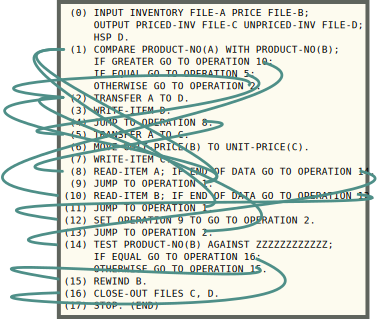
\includegraphics{../images/flow-matic-4.svg}
\caption{spaghetti of goto}
\end{figure}

Hình 3: Sự lộn xộn của lập trình phi cấu trúc

Vấn đề của lập trình phi cấu trúc, hay của \texttt{GOTO}, gồm:

\begin{enumerate}
\def\labelenumi{\arabic{enumi}.}
\item
  Khó nắm bắt luồng chương trình

  Khi đã chạy \texttt{GOTO}, các lệnh phía sau nó không biết khi nào mới
  chạy, vì chương trình chuyển sang lệnh khác mà không trở lại. Luồng
  chạy trở thành một đống ``mì trộn'' như Hình 3, thay vì tuần tự từ
  trên xuống. Tệ hơn, tính trừu tượng bị phá vỡ: khi gọi hàm, thay vì có
  thể bỏ qua chi tiết bên trong, ta phải biết rõ để xem có lệnh nhảy bất
  ngờ nào không.
\item
  Không cài đặt được các chức năng mới (ngoại lệ, quản lí tài nguyên tự
  động,\ldots)

  Xét ví dụ Java sau về quản lí tài nguyên tự động:

\begin{Shaded}
\begin{Highlighting}[]
\ControlFlowTok{try} \OperatorTok{(}\BuiltInTok{Scanner}\NormalTok{ scanner }\OperatorTok{=} \KeywordTok{new} \BuiltInTok{Scanner}\OperatorTok{(}\KeywordTok{new} \BuiltInTok{File}\OperatorTok{(}\StringTok{"f.txt"}\OperatorTok{)))} \OperatorTok{\{}
    \ControlFlowTok{goto}\OperatorTok{(}\NormalTok{SOMEWHERE}\OperatorTok{);}    \CommentTok{// Giả sử Java có GOTO}
\OperatorTok{\}}
\end{Highlighting}
\end{Shaded}

  Do không trả lại luồng điều khiển, việc đóng luồng nhập từ tệp cũng
  không chắc chắn xảy ra, dẫn đến rò rỉ tài nguyên, làm khối lệnh vô
  dụng.

  Điều gần tương tự cũng khiến việc xử lí ngoại lệ và nhiều tính năng
  khác trở nên rất khó đạt được, một khi ngôn ngữ cho phép
  \texttt{GOTO}.
\end{enumerate}

Lập trình cấu trúc đơn giản hóa luồng chạy bằng cách giới hạn các lệnh
nhảy còn \texttt{if}, \texttt{for} và gọi hàm. Khác biệt mấu chốt so với
\texttt{GOTO} là chúng \emph{trả luồng điều khiển} về điểm gọi, thể hiện
rõ ở Hình 4. Theo định nghĩa, ba lệnh trên giải quyết được hậu quả 1.
Đồng thời, hậu quả 2 cũng được giải quyết, do ngôn ngữ đã có cấu trúc
(cụ thể là có call stack).

\begin{figure}
\centering
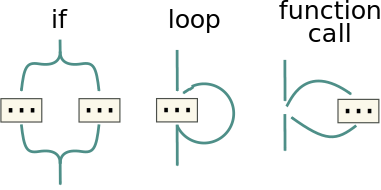
\includegraphics{../images/control-schematics.svg}
\caption{3 basic constructs}
\end{figure}

Hình 4: Ba cấu trúc cơ bản: rẽ nhánh \texttt{if}, lặp \texttt{for} và
gọi hàm

Ngày nay, ba cấu trúc trên là phần không thể thiếu trong mọi ngôn ngữ
lập trình, còn \texttt{GOTO} chỉ dùng trong hợp ngữ. Quá khứ cho thấy
nếu áp dụng một số cấu trúc, giới hạn, ta có thể giải quyết vấn đề một
cách tinh tế và gọn gàng. Trong trường hợp này, SC có thể loại bỏ một số
điểm yếu của các API tương tranh/bất đồng bộ truyền thống, giống cách
lập trình cấu trúc đã làm.

\hypertarget{uxe1p-dux1ee5ng-vuxe0o-hiux1ec7n-tux1ea1i-tux1b0ux1a1ng-tranh-cux1ea5u-truxfac}{%
\subparagraph{2.2.1.3. Áp dụng vào hiện tại: tương tranh cấu
trúc}\label{uxe1p-dux1ee5ng-vuxe0o-hiux1ec7n-tux1ea1i-tux1b0ux1a1ng-tranh-cux1ea5u-truxfac}}

Trước hết, ta xem xét hai kiểu API tương tranh hay dùng hiện nay:

\begin{longtable}[]{@{}
  >{\raggedright\arraybackslash}p{(\columnwidth - 4\tabcolsep) * \real{0.21}}
  >{\raggedright\arraybackslash}p{(\columnwidth - 4\tabcolsep) * \real{0.50}}
  >{\raggedright\arraybackslash}p{(\columnwidth - 4\tabcolsep) * \real{0.29}}@{}}
\toprule
Tên & Giải thích & Ví dụ \\
\midrule
\endhead
Tương tranh & Chạy một hàm theo cách tương tranh với luồng chạy hiện tại
& \texttt{Thread(target=fn).start()\ \#\ Python} \\
Bất đồng bộ & Chạy một hàm khi có sự kiện xảy ra (callback) &
\texttt{element.onclick\ =\ cb;\ //\ JS} \\
\bottomrule
\end{longtable}

Bảng 1: Hai kiểu API tương tranh thường thấy.

Qua Hình 5, không khó để thấy rằng mọi vấn đề của lập trình phi cấu trúc
đều lặp lại với hai API trên:

\begin{figure}
\centering

\includegraphics{../images/sequential-and-go-to-schematic.svg}
\caption{non-structured concurrency}
\end{figure}

Hình 5: Tương tranh phi cấu trúc với \texttt{goroutine} - API kiểu tương
tranh.

\begin{itemize}
\item
  Ta xem lại ví dụ quản lí tài nguyên tự động. Nếu có một luồng thực thi
  khác tương tranh với luồng chính, thì khi luồng chính đóng
  \texttt{Scanner}, có thể luồng kia vẫn đang đọc nó. Vấn đề giờ là đọc
  sau khi đóng. Do đó, tính năng này không thể hoạt động.
\item
  Với tính năng bắt ngoại lệ, nếu có ngoại lệ ở luồng tương tranh, ta
  cũng không có cách nào để biết, và buộc phải kệ nó.
\end{itemize}

Trên thực tế, có thể cài đặt chức năng trên với API hiện tại, tuy vậy đó
đều là cách xử lí riêng, bất tiện. Ví dụ, ES6 có \texttt{catch()} để bắt
ngoại lệ trong \texttt{Promise} mà không (thể) dùng cấu trúc
\texttt{try-catch} sẵn có. Với SC, các vấn đề này đều được giải quyết.

Ta xét một đoạn mã tương tranh dùng coroutine trong Kotlin, tức dùng SC
(không phải coroutine trong mọi ngôn ngữ đều dùng mô hình này):

\begin{figure}
\centering
\includegraphics{../images/kotlin-coroutine.svg}
\caption{kotlin coroutine}
\end{figure}

Hình 6: Tương tranh cấu trúc dùng coroutine trong Kotlin

Đoạn mã trong Hình 6 làm những việc sau:

\begin{itemize}
\item
  Hàm \texttt{launch()} tạo ra các coroutine:

  \begin{itemize}
    \item
    \texttt{launch()} đầu tiên tạo ra coroutine \emph{cha}
  \item
    \texttt{launch()} thứ hai tạo ra coroutine \emph{con}, chạy hàm
    \texttt{A()}
  \item
    Tương tự, có một coroutine con chạy hàm \texttt{B()}
  \end{itemize}
\item
  3 coroutine chạy ``song song'', chính xác hơn là tương tranh
\end{itemize}

Nguyên tắc của SC là: \emph{coroutine cha chờ mọi coroutine con chạy
xong}, kể cả khi nó xong trước. Nguyên tắc này đảm bảo rằng khi một hàm
kết thúc, không còn tác vụ tương tranh nữa, và luồng điều khiển hợp nhất
được trả về điểm gọi. Đột nhiên, hai tính năng có vấn đề ở trên lại hoạt
động:

\begin{itemize}
\item
  Quản lí tài nguyên tự động: do đảm bảo trả luồng điều khiển, tài
  nguyên đảm bảo được đóng; do không còn tác vụ con, tài nguyên không bị
  đọc sau đóng.
\item
  Bắt ngoại lệ: do cấu trúc cha-con (khác với các API hiện tại cho rằng
  hai tác vụ tương tranh là ngang hàng), coroutine con có thể ném ngoại
  lệ để coroutine cha bắt.
\end{itemize}

Chú ý là các API hiện tại không phải không làm được nguyên tắc trên, vấn
đề là thực hiện một cách \emph{tự động} và \emph{đảm bảo}. Ví dụ, trong
JS, để tuân theo SC, ta phải nhớ \texttt{await} với mọi hàm
\texttt{async}. Do không có ràng buộc chặt chẽ này, các tính năng ngôn
ngữ mới cũng khó cài đặt như đã phân tích.

Do trong các ngôn ngữ khác, nguyên tắc trên chỉ là một ca sử dụng, việc
ép buộc viết theo ca sử dụng này đòi hỏi lập trình viên thay đổi suy
nghĩ về tương tranh. Đổi lại, chương trình trở nên sáng rõ, giống những
đoạn mã viết theo kiểu tuần tự truyền thống.

Một khi vấn đề tương tranh được giải quyết hoặc đơn giản hóa, việc song
song hóa (paralellization) để tăng tốc ứng dụng chỉ còn là một chi tiết
cài đặt.

\hypertarget{tuxf3m-tux1eaft}{%
\subparagraph{2.2.1.4. Tóm tắt}\label{tuxf3m-tux1eaft}}

Coroutine với SC là một trong những tính năng quan trọng nhất của
Kotlin, giúp tăng tốc những đoạn mã chạy chậm trong yacv. Mấu chốt của
SC được tóm gọn trong Hình 6. Dù khá mới (Martin Sústrik, tác giả của
ZeroMQ, nêu ý tưởng này năm 2016), mô hình này được cải thiện liên tục,
có thư viện ở nhiều ngôn ngữ như Java (Loom), Python (Trio),\ldots{}
Điều này cho thấy ý tưởng có ý nghĩa lớn, giúp đơn giản hóa tư duy về
tương tranh.

\hypertarget{mux1eabu-thiux1ebft-kux1ebf-mvvm-vuxe0-kiux1ebfn-truxfac-khuyuxean-duxf9ng}{%
\subsubsection{\texorpdfstring{2.3. Mẫu thiết kế MVVM và Kiến trúc
khuyên dùng
}{2.3. Mẫu thiết kế MVVM và Kiến trúc khuyên dùng }}\label{mux1eabu-thiux1ebft-kux1ebf-mvvm-vuxe0-kiux1ebfn-truxfac-khuyuxean-duxf9ng}}

\hypertarget{mux1eabu-thiux1ebft-kux1ebf-mvvm}{%
\paragraph{\texorpdfstring{2.3.1. Mẫu thiết kế MVVM
}{2.3.1. Mẫu thiết kế MVVM }}\label{mux1eabu-thiux1ebft-kux1ebf-mvvm}}

Cũng như các tác vụ lập trình khác, lập trình giao diện sử dụng nguyên
lý Separation of Concern, hiểu đơn giản là chia tách chức năng. Nhiều
năm kinh nghiệm cho thấy giao diện nên được chia làm hai phần chính tách
biệt nhau:

\begin{itemize}
\item
  Model: dữ liệu để hiển thị (trả lời câu hỏi ``cái gì''); liên quan đến
  đối tượng, mảng,\ldots{}
\item
  View: cách để hiển thị dữ liệu đó (trả lời câu hỏi ``như thế nào'');
  liên quan đến các yếu tố giao diện như nút, danh sách,\ldots{}
\end{itemize}

Sự tách biệt thể hiện ở chỗ Model không được biết View. Khi này, giao
diện và nghiệp vụ có thể phát triển khá độc lập với nhau, giúp giảm thời
gian phát triển. Ngược lại, View có biết Model không là tùy vào cách
triển khai cụ thể. Có sự bất đối xứng này là do View luôn liên quan chặt
chẽ đến framework, khác với Model thường đơn giản.

Khó khăn ở đây là làm sao để kết nối hai thành phần riêng biệt kia.
Nhiều mô hình cố giải quyết vấn đề này, tiêu biểu là MVC, MVP và MVVM.
Ta lần lượt xem xét chúng để thấy rằng MVVM phù hợp nhất với Android, do
đó được chọn làm nền tảng cho Kiến trúc Google khuyên dùng.

\hypertarget{mvc-model---view---controller}{%
\subparagraph{2.3.1.1. MVC: Model - View -
Controller}\label{mvc-model---view---controller}}

Phương hướng đầu tiên được thử là MVC, vốn phổ biến vào thời điểm
Android ra đời. Do được phát minh từ lâu và mỗi framework lại có cách
giải thích khác nhau, nên không có một mô hình cụ thể về cách ba thành
phần trên tương tác. Tuy vậy, vẫn có vài điểm chung không đổi:

\begin{enumerate}
\def\labelenumi{\arabic{enumi}.}
\item
  Controller nhận thao tác người dùng
\item
  Sau đó, controller cập nhật Model và View
\end{enumerate}

Ngay ở đây, ta đã thấy điểm yếu của MVC khi áp dụng vào Android. Trong
Android, ứng dụng sử dụng Activity và Fragment để viết giao diện. Hai
đối tượng này cũng kiêm luôn việc nhận thao tác người dùng, tức chúng là
\emph{cả View và Controller}. Mục đích tách ra ba đối tượng do đó không
thể làm được.

Hiện nay, MVC trên Android được coi là lỗi thời, không phù hợp.

\hypertarget{mvp-model---view---presenter}{%
\subparagraph{2.3.1.2. MVP: Model - View -
Presenter}\label{mvp-model---view---presenter}}

Năm 2012, Robert Martin ``Uncle Bob'' xuất bản một bài viết nổi tiếng về
kiến trúc phần mềm: Clean Architecture. MVP, vốn được phát triển từ lâu,
được đông đảo lập trình viên chọn để triển khai Clean Architecture trên
Android. Trước khi Google chọn MVVM, đây là hướng đi mới, có kì vọng cao
sau nhiều thất bại trong việc đưa MVC vào Android.

Nhiệm vụ của ba thành phần như sau:

\begin{itemize}
\item
  Model: vẫn như trong MVC
\item
  View: hiển thị dữ liệu; nhận tương tác người dùng để chuyển sang
  Presenter
\item
  Presenter: trung gian giữa Model và View: nhận tương tác từ View,
  gọi/thay đổi Model, cập nhật View
\end{itemize}

\begin{figure}
\centering
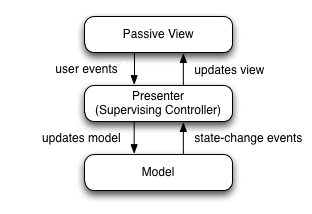
\includegraphics{../images/Model_View_Presenter_GUI_Design_Pattern.png}
\caption{mvp}
\end{figure}

Hình 7: Kiến trúc MVP

Ta thấy điểm yếu View-Controller nhập nhằng được khắc phục, khi View
kiêm luôn việc nhận tương tác. Đồng thời, Model và View hoàn toàn không
biết nhau, đúng theo nguyên lý tách lớp của Clean Architecture.

Ta xét một ứng dụng ToDo đơn giản, trong đó các công việc có thể được
đánh dấu đã hoàn thành. Trong ứng dụng, màn hình hiển thị số việc đã và
chưa hoàn thành. Trong màn hình đó, tương tác của MVP như sau:

\begin{enumerate}
\def\labelenumi{\arabic{enumi}.}
\item
  Presenter lấy tất cả công việc trong Model
\item
  Presenter đếm số việc hoàn thành, chưa hoàn thành
\item
  Presenter gọi hàm của View, truyền hai số đếm được ở trên vào
\end{enumerate}

Đến đây, thiết kế đã khá hoàn chỉnh và phù hợp với Android.

\hypertarget{mvvm-model---view---view-model}{%
\subparagraph{2.3.1.3. MVVM: Model - View - View
Model}\label{mvvm-model---view---view-model}}

\begin{figure}
\centering
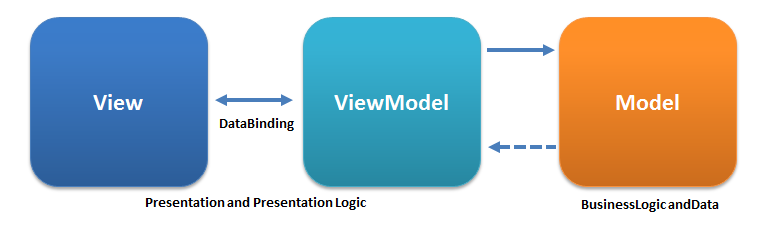
\includegraphics{../images/MVVMPattern.png}
\caption{mvvm}
\end{figure}

Hình 8: Kiến trúc MVVM

Ta quay về chủ đề chính: MVVM. MVVM giống MVP ở chỗ View Model (từ đây
gọi tắt là VM) kết nối View và Model như Presenter. Điểm khác biệt là
cách truyền dữ liệu:

\begin{itemize}
\item
  Trong MVP, Presenter gọi hàm của View để truyền dữ liệu cho View
\item
  Trong MVVM, VM dùng \emph{data binding} để truyền dữ liệu cho View
\end{itemize}

Data binding là cơ chế để \emph{tự động} đưa dữ liệu vào thành phần hiển
thị. Quay lại ví dụ ToDo ở trên, nếu dùng data binding để ``gắn'' (bind)
danh sách công việc vào View, thì khi danh sách thay đổi, View cũng tự
động thay đổi theo.

Do dùng data binding thay vì gọi hàm thủ công, VM không cần có tham
chiếu tới View, khác với Presenter. Điều này giúp liên kết View - VM
thêm \emph{lỏng lẻo} (loose coupling), giúp kiểm thử dễ dàng hơn. Phần
còn lại của hai mô hình giống nhau: View cần biết VM để chuyển tương
tác; VM cần biết Model để lấy dữ liệu.

Do là mô hình phù hợp nhất trong cả ba với riêng Android, MVVM được chọn
làm nền tảng cho Kiến trúc Google khuyên dùng.

\hypertarget{kiux1ebfn-truxfac-google-khuyuxean-duxf9ng}{%
\paragraph{\texorpdfstring{2.3.2. Kiến trúc Google khuyên dùng
}{2.3.2. Kiến trúc Google khuyên dùng }}\label{kiux1ebfn-truxfac-google-khuyuxean-duxf9ng}}

Kiến trúc Google khuyên dùng có gốc là mô hình MVVM, có dạng như Hình 9:

\begin{figure}
\centering
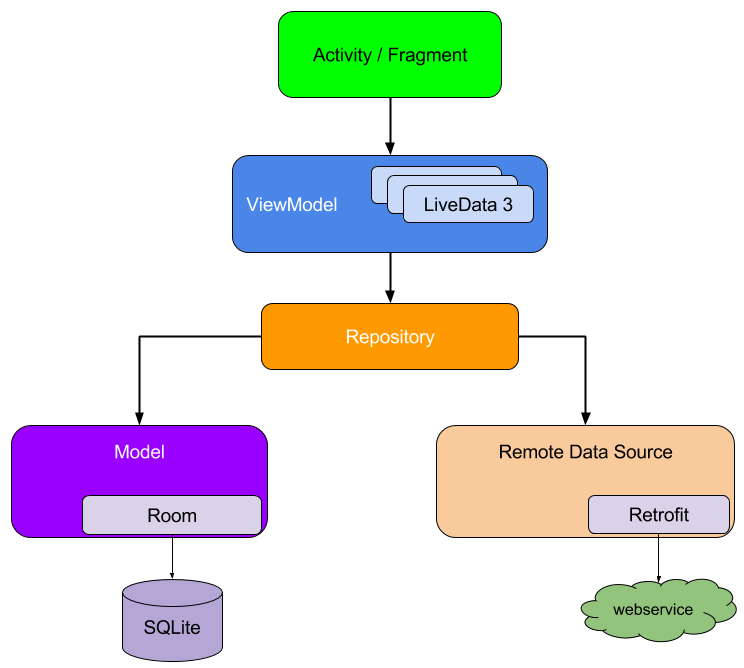
\includegraphics{../images/final-architecture.png}
\caption{Google recommended architecture}
\end{figure}

Hình 9: Kiến trúc Google khuyên dùng

\begin{itemize}
\item
  Repository là Model trong MVVM, giúp VM lấy dữ liệu mà không cần quan
  tâm dữ liệu lấy từ đâu: cơ sở dữ liệu, gọi API qua mạng,\ldots{}
\item
  LiveData là cơ chế data binding dùng luồng dữ liệu (stream)
\item
  Activity/Fragment là View
\end{itemize}

Repository là một điểm được chi tiết hóa so với MVVM. Google cho rằng
một ứng dụng không nên hoàn toàn vô dụng nếu không có mạng. Do đó, cần
có hai nguồn dữ liệu: dữ liệu từ máy chủ, và dữ liệu đệm, ngoại tuyến.
Khi có nhiều nguồn dữ liệu, mẫu thiết kế Repository là lựa chọn hiển
nhiên để trừu tượng hóa chúng.

yacv sử dụng kiến trúc này, dù không có tính năng liên quan đến mạng. Lý
do là yacv có tính năng quét truyện hoạt động chậm giống như giao tiếp
mạng, nên cần dữ liệu đệm và dữ liệu quét thực tế.

\hypertarget{cux1a1-sux1edf-dux1eef-liux1ec7u-sqlite}{%
\subsubsection{\texorpdfstring{2.4. Cơ sở dữ liệu SQLite
}{2.4. Cơ sở dữ liệu SQLite }}\label{cux1a1-sux1edf-dux1eef-liux1ec7u-sqlite}}

SQLite là một hệ quản trị cơ sở dữ liệu quan hệ (RDBMS). Từ ``Lite''
trong tên có nghĩa là ``nhỏ'', thể hiện mục tiêu thiết kế chính của nó
là nhỏ gọn. SQLite có thể được nhúng vào phần mềm khác ở dạng thư viện,
thay vì là một phần mềm riêng với cấu trúc chủ-khách như MySQL,\ldots{}
Ngay từ những phiên bản đầu, Android đã tích hợp SQLite, giúp lập trình
viên không phải nhúng SQLite vào từng ứng dụng.

Để đạt mục tiêu, SQLite chỉ giữ các tính năng SQL cốt lõi
(tạo/đọc/sửa/xóa), giao dịch (có ACID), và chỉ tối ưu cho việc truy cập
từ một ứng dụng cùng lúc. Các tính năng thường có trong RDBMS cho máy
chủ, như nhân bản (replication), chia dữ liệu tự động (sharding), khóa
dòng, đọc ghi nhiều luồng cùng lúc,\ldots{} được loại bỏ. Do đó, với nhu
cầu lưu trữ đơn giản, SQLite vừa nhanh vừa gọn.

yacv dùng SQLite để lưu đệm thông tin truyện, tránh quét nhiều lần.

\hypertarget{thux1b0-viux1ec7n-orm-room}{%
\paragraph{\texorpdfstring{2.4.1. Thư viện ORM Room
}{2.4.1. Thư viện ORM Room }}\label{thux1b0-viux1ec7n-orm-room}}

Room là một thư viện thuộc Jetpack. Đây có thể xem là một thư viện ORM
đơn giản cho SQLite. Room tự động làm nhiều công việc liên quan đến SQL:

\begin{itemize}
\item
  Tạo bảng: Người viết chỉ cần khai báo các đối tượng dữ liệu như một
  lớp (class) thông thường, rồi đánh dấu với Annotation và interface của
  Room. Sau đó, Room sinh các bảng tương ứng.
\item
  Truy vấn: Người viết chỉ cần viết lệnh SQL. Sau đó, Room sinh hàm truy
  vấn tương ứng, chuyển dữ liệu dạng đối tượng sang dạng để lưu trong
  bảng và ngược lại.
\item
  Kiểm tra truy vấn khi biên dịch: Dò lỗi lệnh SQL mà không cần chờ đến
  khi chạy.
\item
  Kiểm soát lược đồ (schema): Khi thêm/sửa/xóa bảng/cột, Room luôn phát
  hiện và ép viết cơ chế cập nhật. Do đó, ứng dụng dùng lược đồ cũ khi
  được cập nhật sẽ biết cách sửa cơ sở dữ liệu đến phiên bản lược đồ
  mới.
\item
  Tương thích với LiveData: Giúp View cập nhật theo cơ sở dữ liệu.
\end{itemize}

\hypertarget{tuxecm-kiux1ebfm-vux103n-bux1ea3n}{%
\paragraph{\texorpdfstring{2.4.2. Tìm kiếm văn bản
}{2.4.2. Tìm kiếm văn bản }}\label{tuxecm-kiux1ebfm-vux103n-bux1ea3n}}

Tìm kiếm văn bản (full-text search, hay gọi tắt là FTS) là một trong số
ít các tính năng nâng cao được giữ lại trong SQLite. Cũng như các thư
viện tìm kiếm khác, SQLite cài đặt chức năng này bằng chỉ mục đảo
(inverted index) - một cấu trúc giống từ điển:

\begin{enumerate}
\def\labelenumi{\arabic{enumi}.}
\item
  Khi dữ liệu văn bản được ghi, nó được tách thành các từ.
\item
  Các từ được đưa vào chỉ mục đảo: khóa là từ đó, giá trị là khóa đại
  diện \texttt{rowid}.
\end{enumerate}

FTS khác với đánh chỉ mục thường (cũng là chỉ mục đảo nhưng cho kiểu dữ
liệu thông thường) ở bước 1: \emph{từng từ} được tách ra, còn chỉ mục
thường dùng \emph{cả} văn bản. Do đó, khi tìm từ lẻ, FTS có thể tìm hàng
có từ đó rất nhanh. Điểm yếu là ghi chậm, kích cỡ lớn hơn chỉ mục
thường. Nếu bản thân dữ liệu văn bản trong cột là một khối, ví dụ như
email, chỉ mục thường đã đủ tốt, không cần FTS. Ngoài ra, nếu muốn, ở
bước này có thể dùng kĩ thuật rút gọn từ (stemming; chỉ đúng với tiếng
Anh), giúp tìm kiếm linh động hơn.

Trong SQLite, một số kĩ thuật xử lí ngôn ngữ tự nhiên cơ bản cũng được
áp dụng trong bước 1, như rút gọn từ (stemming, dùng thuật toán Porter,
ví dụ khi tìm ``run'' sẽ ra được cả ``runs'', ``running'', ``ran''; tất
nhiên chỉ đúng với tiếng Anh), giúp kết quả tìm kiếm linh động hơn.

yacv có tính năng tìm kiếm tiêu đề, tên nhân vật,\ldots{} đều là những
câu văn, đoạn văn. Do đó, FTS có vai trò không thể thiếu để tăng tốc tìm
kiếm trong ứng dụng.

\hypertarget{ux111ux1ecbnh-dux1ea1ng-tux1ec7p-nuxe9n-zip-vuxe0-cbz}{%
\subsubsection{\texorpdfstring{2.5. Định dạng tệp nén ZIP và CBZ
}{2.5. Định dạng tệp nén ZIP và CBZ }}\label{ux111ux1ecbnh-dux1ea1ng-tux1ec7p-nuxe9n-zip-vuxe0-cbz}}

Các tệp truyện mà yacv đọc có định dạng CBZ, bản chất chính là tệp nén
ZIP. Do yêu cầu của các phần sau, định dạng tệp ZIP cũng cần được trình
bày ở mức cơ bản.

\hypertarget{ux111ux1ecbnh-dux1ea1ng-tux1ec7p-nuxe9n-zip}{%
\paragraph{\texorpdfstring{2.5.1. Định dạng tệp nén ZIP
}{2.5.1. Định dạng tệp nén ZIP }}\label{ux111ux1ecbnh-dux1ea1ng-tux1ec7p-nuxe9n-zip}}

ZIP là một định dạng tệp nén không mất mát (lossless). Được phát minh
vào năm 1989 bởi Phil Katz, ZIP đã trở thành định dạng nén tiêu chuẩn,
được hỗ trợ trên gần như mọi nền tảng, bao gồm Android.

ZIP thực chất là một định dạng chứa (container), chuyên chứa dữ liệu
nén, chứ không phải thuật toán nén; thuật toán nén hay dùng nhất trong
ZIP là DEFLATE. Một trong các mục tiêu của ZIP là giúp việc sửa tệp nén
(thêm, sửa, xóa tệp con trong tệp ZIP) nhanh nhất có thể. Mục tiêu đó
dẫn đến thiết kế sau, được thể hiện trong Hình 10:

\begin{itemize}
\item
  Thuật toán nén mỗi tệp gốc thành một tệp nhị phân, ở đây gọi là
  \emph{tệp nén lẻ} (data trong Hình 10). Sau đó, các tệp nén lẻ này
  được nối thành tệp ZIP cuối cùng.
\item
  Ở đầu mỗi tệp nén lẻ là một header gọi là \emph{File Entry} để lưu
  thông tin liên quan, trong đó có \emph{tên tệp gốc} và \emph{vị trí
  bắt đầu} (offset), tức số byte tính từ đầu tệp ZIP đến tệp nén lẻ
  tương ứng.
\item
  Ở \emph{cuối} tệp ZIP, sau khi đã nối các tệp nén lẻ cùng header lại,
  các header được gom lại, lưu một lần nữa vào một cấu trúc gọi là
  \emph{Central Directory}. Có thể so sánh File Entry như các \emph{đề
  mục}, còn Central Directory là \emph{mục lục}.
\item
  Hai thông tin quan trọng trong File Entry là tên tệp gốc và \emph{vị
  trí bắt đầu} (offset), tức số byte tính từ đầu tệp ZIP đến tệp nén lẻ
  tương ứng.
\end{itemize}

\begin{figure}
\centering
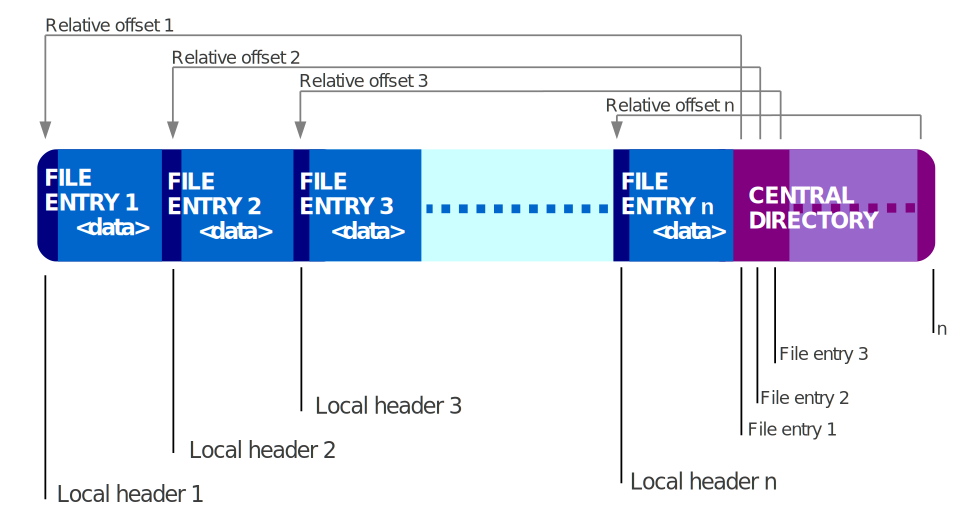
\includegraphics{../images/ZIP-64_Internal_Layout.svg}
\caption{zip file layout}
\end{figure}

Hình 10: Cấu trúc tệp nén ZIP

Ta phân tích kĩ hơn:

\begin{itemize}
\item
  Do nén riêng từng tệp, có thể dùng thuật toán khác nhau tối ưu với
  từng tệp.
\item
  Cũng do nén riêng và có mục lục, việc thêm/sửa/xóa (gọi chung là sửa)
  và đọc có thể được thực hiện với từng tệp lẻ, thay vì phải giải nén,
  sửa, rồi nén lại toàn bộ.
\item
  Nhờ mục lục (chứa vị trí tệp nén lẻ), việc sửa còn diễn ra nhanh do
  ứng dụng biết vị trí để đọc ghi dữ liệu.
\item
  Mục lục đặt ở cuối là tối ưu:

  \begin{itemize}
    \item
    Giả sử mục lục đặt ở đầu. Khi sửa, toàn bộ các tệp nén lẻ phải di
    chuyển để tạo chỗ cho mục lục mới (giống như thêm một phần tử vào
    mảng ở vị trí đầu: toàn bộ các phần tử sau bị đẩy lên để tạo chỗ
    trống).
  \item
    Do mục lục nằm ở cuối tệp ZIP, nên khi sửa chỉ cần đẩy các tệp nén
    lẻ từ chỗ sửa. Trước đây tối ưu này rất quan trọng. Do đĩa mềm -
    phương tiện chia sẻ chủ yếu thời đó - có dung lượng nhỏ, tệp ZIP có
    thể phải cắt ra cho vừa. Thiết kế này cho phép chỉ sửa lại dữ liệu ở
    một số đĩa, thay vì toàn bộ.
  \item
    Hơn nữa, nếu mục lục ở đầu thì ngay trong khi nén, các tệp nén lẻ bị
    di chuyển như trên do mục lục liên tục được cập nhật.
  \end{itemize}
\end{itemize}

Tóm lại, cấu trúc tệp nén ZIP cho phép sửa và giải nén từng tệp gốc rất
dễ dàng. Nhiều định dạng tệp nén khác (TAR, 7z,\ldots) không có tính
năng này, do gộp toàn bộ các tệp vào rồi nén một thể. Trong trường hợp
đó, tệp nén được gọi là \emph{đặc} (solid), và rất khó để đọc/sửa tệp
lẻ.

\hypertarget{ux111ux1ecbnh-dux1ea1ng-tux1ec7p-truyux1ec7n-cbz}{%
\paragraph{\texorpdfstring{2.5.2. Định dạng tệp truyện CBZ
}{2.5.2. Định dạng tệp truyện CBZ }}\label{ux111ux1ecbnh-dux1ea1ng-tux1ec7p-truyux1ec7n-cbz}}

Tệp truyện CBZ chỉ là một tệp nén ZIP thông thường, trong đó có:

\begin{itemize}
\item
  Các tệp ảnh trang truyện: Các tệp này là tệp ảnh JPEG, PNG,\ldots{}
  thông thường. Tên tệp được đánh số tăng dần để biểu thị thứ tự trang.
  Tuy nhiên, không có một cấu trúc/định dạng tên tệp nào được thống
  nhất.
\item
  (Tùy chọn) Một tệp metadata: Có nhiều định dạng metadata. Hiện nay,
  yacv chấp nhận định dạng ComicInfo, được trình bày ở
  \protect\hyperlink{P8.2-comicinfo.xsd}{Phụ lục 2}. Định dạng này lưu
  trong một tệp có tên \texttt{ComicInfo.xml}.
\end{itemize}

\begin{center}\rule{0.5\linewidth}{0.5pt}\end{center}

\hypertarget{chux1b0ux1a1ng-3-phuxe2n-tuxedch-yuxeau-cux1ea7u}{%
\subsection{\texorpdfstring{3. Chương 3: Phân tích yêu cầu
}{3. Chương 3: Phân tích yêu cầu }}\label{chux1b0ux1a1ng-3-phuxe2n-tuxedch-yuxeau-cux1ea7u}}

Chương này tìm hiểu đối tượng người dùng nhắm tới để tìm ra \emph{Nhu
cầu} của họ. Nhu cầu này sau đó được phân tích thành các \emph{Yêu cầu
chức năng} và \emph{phi chức năng}. Cuối cùng, các chức năng được mổ xẻ,
mô tả kĩ để được \emph{Đặc tả ca sử dụng}, là bộ khung cho quá trình
phát triển ứng dụng.

\hypertarget{muxf4-tux1ea3-chung}{%
\subsubsection{\texorpdfstring{3.1. Mô tả chung
}{3.1. Mô tả chung }}\label{muxf4-tux1ea3-chung}}

\hypertarget{ngux1b0ux1eddi-duxf9ng}{%
\paragraph{\texorpdfstring{3.1.1. Người dùng
}{3.1.1. Người dùng }}\label{ngux1b0ux1eddi-duxf9ng}}

Ứng dụng yacv tập trung vào một số ít người dùng, là một trong hai nhóm
sau:

\begin{itemize}
\item
  Người dùng sưu tầm truyện
\item
  Người dùng có yêu cầu đọc truyện với chất lượng hình ảnh cao
\end{itemize}

Cả hai nhóm có điểm chung là kĩ tính, yêu cầu cao về trải nghiệm đọc
truyện, cụ thể là về \emph{chất lượng hình ảnh}. Cũng do kĩ tính, nên cả
hai nhóm không cần nhiều chức năng, tuy nhiên từng chức năng cần hoàn
thiện. Nhóm người dùng sưu tầm truyện còn có yêu cầu \emph{xem thông tin
(metadata)} của tệp truyện.

Tóm lại, ta thu được hai \emph{Nhu cầu} của nhóm người dùng hướng đến:

\begin{itemize}
\item
  Đọc truyện trong tệp truyện
\item
  Xem metadata
\end{itemize}

\hypertarget{mux1ee5c-ux111uxedch}{%
\paragraph{\texorpdfstring{3.1.2. Mục đích
}{3.1.2. Mục đích }}\label{mux1ee5c-ux111uxedch}}

Trước khi đi vào chi tiết yêu cầu ở mục tiếp theo, tôi muốn làm rõ mục
đích của sản phẩm đã nhắc ở \protect\hyperlink{P1.1-background}{mục
1.1}.

\begin{itemize}
\item
  Ứng dụng yacv chỉ gồm các tính năng liên quan đến đọc \textbf{truyện
  tranh} và là ứng dụng \textbf{ngoại tuyến} (tức đọc các tệp truyện có
  sẵn trên điện thoại).
\item
  Ứng dụng \emph{không phải} là ứng dụng khách cho các trang đọc truyện
  hiện có, hay có máy chủ tập trung riêng để cung cấp truyện.
\item
  Ứng dụng \emph{không có} khả năng đọc truyện đuôi PDF, cùng với các
  định dạng truyện thiên về chữ khác như TXT, EPUB.
\end{itemize}

Các giới hạn này nhằm tránh cho phần mềm quá phức tạp với tôi, đồng thời
phù hợp (không thừa thiếu chức năng) so với nhu cầu của nhóm người dùng
mục tiêu đã nêu ở \protect\hyperlink{P3.1.1-users}{mục 3.1.1}.

\hypertarget{yuxeau-cux1ea7u-ux111ux1eb7t-ra}{%
\subsubsection{\texorpdfstring{3.2. Yêu cầu đặt ra
}{3.2. Yêu cầu đặt ra }}\label{yuxeau-cux1ea7u-ux111ux1eb7t-ra}}

\hypertarget{yuxeau-cux1ea7u-chux1ee9c-nux103ng}{%
\paragraph{\texorpdfstring{3.2.1. Yêu cầu chức năng
}{3.2.1. Yêu cầu chức năng }}\label{yuxeau-cux1ea7u-chux1ee9c-nux103ng}}

Ứng dụng có các chức năng chính sau:

\begin{itemize}
\item
  Quét các tệp truyện trên thiết bị
\item
  Hiển thị danh sách truyện
\item
  Đọc truyện
\item
  Xem metadata truyện
\item
  Tìm kiếm truyện
\item
  Xóa truyện
\end{itemize}

\hypertarget{yuxeau-cux1ea7u-phi-chux1ee9c-nux103ng}{%
\paragraph{\texorpdfstring{3.2.2. Yêu cầu phi chức năng
}{3.2.2. Yêu cầu phi chức năng }}\label{yuxeau-cux1ea7u-phi-chux1ee9c-nux103ng}}

Ứng dụng cần đạt một số tiêu chí sau:

\begin{itemize}
\item
  \emph{Không trói buộc người dùng} (vendor lock-in): Đây là một tiêu
  chí quan trọng (trên thực tế nó có ảnh hưởng lớn đến thiết kế kĩ thuật
  của yacv). Điểm thể hiện rõ tiêu chí này là truyện phải được lưu trong
  \emph{phân vùng chung}, để ứng dụng nào cũng có thể đọc, thay vì lưu
  trong phân vùng của riêng yacv. Do đó, người dùng có thể xóa, đổi ứng
  dụng bất kì lúc nào.
\item
  Phản hồi nhanh: Các thao tác cần có thời gian phản hồi nhanh. Phản hồi
  nhanh không nhất thiết là thời gian thực thi ngắn, mà là luôn có các
  thông báo tiến độ cho người dùng.

  \begin{itemize}
    \item
    Luôn hiện thông báo chờ khi làm việc gì đó lâu
  \item
    Nếu có nhiều kết quả tìm kiếm, hiển thị từ từ, đưa kết quả đã biết
    lên trước
  \end{itemize}
\item
  Tốc độ xem truyện chấp nhận được: Đây là một phần của phản hồi nhanh,
  nhưng được tách riêng vì độ quan trọng của nó. Tốc độ xem truyện gồm
  hai tiêu chí:

  \begin{itemize}
    \item
    Tốc độ mở truyện, tức tốc độ xem trang đầu (có thể so với first
    contentful paint trong lập trình web)
  \item
    Tốc độ cuộn trang tới-lui
  \end{itemize}
\item
  Chiếm ít bộ nhớ: Bộ nhớ chiếm dụng của ứng dụng gồm hai phần: bộ nhớ
  RAM và bộ nhớ tạm, cả hai cần sử dụng ít dung lượng nhất có thể. Đây
  là một yêu cầu đáng cân nhắc, lí do vì kích cỡ từng tệp truyện thường
  rất lớn (từ vài chục đến hơn một trăm megabyte), tuy nhiên cần chú ý
  cân bằng yêu cầu này với yêu cầu về tốc độ (đánh đổi không gian-thời
  gian).
\item
  Giao diện đơn giản, trực quan: Người dùng hướng đến có thể xếp vào
  nhóm người dùng ``say mê'' (enthusiast), do đó giao diện chỉ cần đơn
  giản rõ ràng, không màu mè, tập trung vào tính năng.
\end{itemize}

\hypertarget{phuxe2n-tuxedch-yuxeau-cux1ea7u}{%
\subsubsection{\texorpdfstring{3.3 Phân tích yêu cầu
}{3.3 Phân tích yêu cầu }}\label{phuxe2n-tuxedch-yuxeau-cux1ea7u}}

Mỗi yêu cầu đã xác định trong
\protect\hyperlink{P3.2.1-functional-requirements}{mục 3.2.1.} được coi
là một ca sử dụng, được trình bày trong các tiểu mục dưới đây.

\emph{Người dùng duy nhất} trong các ca sử dụng là \emph{người đọc}, do
đó hai cụm từ này sẽ được dùng hoán đổi cho nhau. Do ứng dụng hoàn toàn
ngoại tuyến, người đọc cũng không có tương tác với nhau.

Do ứng dụng đơn giản, các ca sử dụng tách biệt, nên mỗi ca sử dụng gắn
với một \emph{màn hình}. Có tổng cộng năm màn hình sẽ được mô tả, gồm:

\begin{itemize}
\item
  Màn hình Thư viện
\item
  Màn hình Thư mục
\item
  Màn hình Đọc truyện
\item
  Màn hình Metadata
\item
  Màn hình Tìm kiếm
\end{itemize}

\hypertarget{quuxe9t-cuxe1c-tux1ec7p-truyux1ec7n-truxean-thiux1ebft-bux1ecb}{%
\paragraph{\texorpdfstring{3.3.1. Quét các tệp truyện trên thiết bị
}{3.3.1. Quét các tệp truyện trên thiết bị }}\label{quuxe9t-cuxe1c-tux1ec7p-truyux1ec7n-truxean-thiux1ebft-bux1ecb}}

\begin{itemize}
\item
  \textbf{Mô tả}:

  Người đọc \emph{chọn} một thư mục trong điện thoại làm thư mục gốc.
  Ứng dụng sẽ \emph{quét} thư mục này và tìm các tệp truyện, rồi hiển
  thị những thư mục chứa tệp truyện cho người đọc chọn.
\item
  \textbf{Luồng chính}:

  \begin{enumerate}
  \def\labelenumi{\arabic{enumi}.}
  \item
    Người đọc bật ứng dụng (tức ở Màn hình Thư viện)
  \item
    Người đọc ấn vào nút thay đổi thư mục gốc.
  \item
    Trình chọn thư mục của Android hiện ra, cho phép người đọc chọn thư
    mục làm thư mục gốc.
  \item
    Màn hình Thư viện trở lại, quét và hiển thị các thư mục chứa truyện
    trong thư mục gốc, đồng thời lưu kết quả quét vào cơ sở dữ liệu.

    Nếu người đọc đã chọn một thư mục gốc, ca sử dụng này \emph{thay
    thế} thư mục gốc đã chọn bằng thư mục vừa chọn.
  \end{enumerate}
\item
  \textbf{Luồng thay thế}:

  Khi người dùng bật ứng dụng, và đã chọn một thư mục gốc từ lần sử dụng
  trước đó, tức ứng dụng cần \emph{quét lại}, khác với Luồng chính là
  \emph{quét mới}:

  \begin{itemize}
    \item
    Người đọc bật ứng dụng (tức ở Màn hình Thư viện).
  \item
    Ứng dụng quét lại truyện trong thư mục gốc, và cập nhật các thay đổi
    vào cơ sở dữ liệu.
  \end{itemize}
\item
  \textbf{Luồng ngoại lệ}:

  Nếu người đọc không chọn thư mục nào, quay lại Màn hình Thư viện và
  không thay đổi gì.

  Nếu có lỗi trong quá trình chọn thư mục, cần gợi ý người đọc chọn lại.
  Lỗi gồm:

  \begin{itemize}
    \item
    Thiếu quyền đọc
  \item
    Không tìm được thư mục gốc
  \item
    Thư mục gốc không có truyện
  \end{itemize}

  Nếu có lỗi trong quá trình quét cần phải giảm thiểu và giấu khỏi người
  đọc.
\item
  \textbf{Kích hoạt khi}:

  Người dùng ấn vào nút thay đổi thư mục gốc.
\item
  \textbf{Điều kiện}:

  \begin{itemize}
  \item
    Tiền điều kiện:

    \begin{itemize}
        \item
      Ứng dụng ở Màn hình Thư viện
    \item
      Nếu là quét lại, cần có thư mục gốc
    \end{itemize}
  \item
    Hậu điều kiện: Ứng dụng ở Màn hình Thư viện

    \begin{itemize}
        \item
      Lưu truyện quét được vào cơ sở dữ liệu. Nếu là quét mới, cần xóa
      hẳn cơ sở dữ liệu cũ. Quét lại thì phải giữ cơ sở dữ liệu sẵn có.
    \item
      Hiển thị thư mục truyện quét được
    \item
      Hiển thị lỗi nếu có (ba loại lỗi ở trên), và gợi ý xử lí
    \end{itemize}
  \end{itemize}
\item
  \textbf{Yêu cầu phi chức năng}:

  Nếu đang quét, Màn hình Thư viện cần hiển thị danh sách thư mục theo
  tiến độ, ứng dụng quét đến đâu hiển thị đến đấy.
\end{itemize}

Đây là ca sử dụng đầu tiên khi người đọc chạy ứng dụng lần đầu. Các tệp
truyện sẽ được quét từ thư mục gốc, rồi được gom lại theo thư mục như mô
tả ở \protect\hyperlink{P3.3.2-browsing}{ca sử dụng kế tiếp}.

Màn hình đầu tiên khi người đọc bật lên gọi là \emph{Màn hình Thư viện}
(Library screen). Các thư mục chứa truyện, hoặc thông báo lỗi liên quan
đến bản thân quá trình chọn truyện (đã miêu tả trong bước 6 ở trên) sẽ
được hiển thị ở màn hình này.

Ca sử dụng này có luồng thay thế là trường hợp quét tự động chạy mỗi khi
khi chạy ứng dụng mà không cần người dùng kích hoạt.

Khi quét, ứng dụng phải đọc luôn cả metadata của tệp truyện nếu có. Các
trường trong metadata được giải thích chi tiết trong
\protect\hyperlink{P8.1-metadata}{Phụ lục 1}. Hiện nay, yacv chấp nhận
định dạng metadata ComicInfo, là một tệp XML trong tệp truyện.
\protect\hyperlink{P8.2-comicinfo.xsd}{Phụ lục 2} trình bày lược đồ XSD
của định dạng metadata này.

Một số metadata có thể được trích xuất ngay từ tên tệp truyện. Do không
có quy chuẩn trong việc đặt tên tệp, cách trích xuất này không ổn định,
tuy nhiên cũng không phải ý tưởng tồi. Nếu có thể, dựa vào
\protect\hyperlink{P8.1-metadata}{Phụ lục 1} để thử trích xuất từ tên
tệp truyện.

Tới đây người đọc có thể thực hiện các ca sử dụng khác, trong đó quan
trọng nhất là duyệt theo thư mục rồi xem truyện.

\hypertarget{duyux1ec7t-truyux1ec7n}{%
\paragraph{\texorpdfstring{3.3.2. Duyệt truyện
}{3.3.2. Duyệt truyện }}\label{duyux1ec7t-truyux1ec7n}}

\begin{itemize}
\item
  \textbf{Mô tả}:

  Ứng dụng hiển thị những thư mục chứa tệp truyện, khi ấn vào sẽ hiển
  thị tệp truyện trong thư mục đó.
\item
  \textbf{Luồng chính}:

  \begin{enumerate}
  \def\labelenumi{\arabic{enumi}.}
    \item
    Người đọc bật ứng dụng (tức ở Màn hình Thư viện).
  \item
    Người đọc duyệt danh sách thư mục truyện, và chọn một thư mục.
  \item
    Người đọc duyệt danh sách truyện trong thư mục.
  \end{enumerate}
\item
  \textbf{Kích hoạt khi}:

  Người dùng bật ứng dụng.
\item
  \textbf{Điều kiện}:

  \begin{itemize}
    \item
    Tiền điều kiện: Ứng dụng đã quét được ít nhất một thư mục chứa
    truyện.
  \item
    Hậu điều kiện: Ứng dụng ở Màn hình Thư mục.
  \end{itemize}
\item
  \textbf{Yêu cầu phi chức năng}:

  Nếu đang quét, Màn hình Thư viện cần hiển thị danh sách thư mục theo
  tiến độ, ứng dụng quét đến đâu hiển thị đến đấy.

  Mỗi thư mục cần hiển thị:

  \begin{itemize}
    \item
    Tên thư mục
  \item
    Ảnh đại diện cho thư mục: bìa một truyện bất kì tìm được trong thư
    mục
  \end{itemize}

  Mỗi tệp truyện cần hiển thị:

  \begin{itemize}
    \item
    Tên truyện
  \item
    Bìa truyện
  \item
    Tiến độ đọc
  \item
    Đánh giá yêu thích
  \end{itemize}
\end{itemize}

Đây là ca sử dụng đầu tiên cho phép người dùng duyệt truyện, là một
trong hai ca sử dụng mặc định khi người dùng mở ứng dụng (cùng với ca sử
dụng quét lại). Ca sử dụng này liên quan đến hai màn hình.

Màn hình đầu tiên khi người đọc bật lên gọi là \emph{Màn hình Thư viện}
(Library screen). Màn hình này hiển thị các thư mục chứa truyện, hoặc
thông báo lỗi nếu có của quá trình quét truyện (đã mô tả ở Luồng ngoại
lệ của \protect\hyperlink{P3.3.1-scan}{mục trước}).

Màn hình khi người đọc chọn một thư mục gọi là \emph{Màn hình Thư mục}
(Directory screen). Màn hình này hiển thị các tệp truyện trong thư mục
đó.

Trong yacv, truyện được quản lí và duyệt theo thư mục. Lí do cho lựa
chọn thiết kế này là vì các phương pháp duyệt khác không trực quan:

\begin{itemize}
\item
  Các phương pháp duyệt khác chỉ bao gồm duyệt theo metadata, tức duyệt
  theo các thông tin đi kèm như Tác giả, Nhân vật, Bộ truyện,\ldots{}
  thì yêu cầu truyện phải có đủ metadata. Trên thực tế, không phải tệp
  truyện nào cũng có đủ thông tin này, do vậy sẽ có trường hợp rất nhiều
  truyện bị gom vào mục ``Không đủ thông tin''. Hơn nữa, giả sử truyện
  có đi kèm metadata, ta xem xét tiếp trường hợp dưới.
\item
  Giả sử ta quản lí theo Nhân vật: Vậy để trực quan, yacv phải hiển thị
  ảnh nhân vật. Hiện nay, việc nhận diện và cắt đúng ảnh phần mặt nhân
  vật ra để tạo ảnh đại diện có thể nói là bất khả thi. Do vậy, khi
  duyệt theo Nhân vật, người đọc chỉ có thể thấy tên, không thấy một
  hình ảnh gợi ý nào khác, dẫn đến khó khăn khi sử dụng. Lập luận tương
  tự có thể dùng với các cách xếp khác.
\item
  Một cách xếp có thể nói là tốt là xếp theo Bộ truyện, tuy nhiên ta lại
  quay về vấn đề thiếu metada.
\end{itemize}

Hơn nữa, các thư mục cần được ``làm phẳng'', tức là hiển thị thư mục con
(cháu,\ldots) ngang hàng với thư mục gốc. Ví dụ sau cho thấy cách yacv
làm phẳng cây thư mục:

\begin{verbatim}
| Cây thư mục gốc                   | yacv đã làm phẳng         |
|-----------------------------------|---------------------------|
| thư mục gốc                       | thư mục gốc               |
| ├── Original Sin #1.cbz           | └── Original Sin #1.cbz   |
| └── House of M                    | House of M                |
|     ├── House of M #1.cbz         | ├── House of M #1.cbz     |
|     ├── House of M #3.cbz         | └── House of M #3.cbz     |
|     └── Tie-ins                   | Tie-ins                   |
|         └── Black Panther #7.cbz  | └── Black Panther #7.cbz  |
\end{verbatim}

Bảng 2: Cách yacv làm phẳng thư mục

Theo như bảng trên, các màn hình trong yacv được tổ chức như sau:

\begin{itemize}
\item
  Màn hình Thư viện: có 3 thư mục:

  \begin{itemize}
    \item
    thư mục gốc
  \item
    House of M
  \item
    Tie-ins
  \end{itemize}
\item
  Khi chọn ``House of M'': chuyển sang Màn hình Thư mục tương ứng, không
  có thư mục con, và có 2 tệp truyện:

  \begin{itemize}
    \item
    House of M \#1.cbz
  \item
    House of M \#3.cbz
  \end{itemize}
\item
  Tương tự với các thư mục khác.
\end{itemize}

Có ba lí do cho lựa chọn thiết kế này:

\begin{itemize}
\item
  Giảm độ phức tạp khi lập trình.
\item
  Người đọc không phải đi qua nhiều tầng thư mục để đến được tệp truyện
  cần đọc.
\item
  Không có ca sử dụng có ý nghĩa cho thư mục lồng nhau:

  Trường hợp hợp lí nhất cho việc có thư mục lồng nhau là khi lưu các
  tệp truyện liên quan đến một bộ truyện (tie-ins), như cột trái Bảng 2:

  \begin{itemize}
    \item
    Thư mục cha (House of M) chứa tệp truyện trong bộ truyện cùng tên và
    thư mục tie-ins.
  \item
    Thư mục Tie-ins chứa các tệp truyện tie-in.
  \end{itemize}

  Tuy nhiên, bản thân các tệp tie-in lại là tệp truyện thông thường
  trong một bộ truyện khác, do đó nếu tổ chức thư mục như thế này sẽ dẫn
  đến tình trạng lặp tệp truyện, là điều không mong muốn ngay cả với máy
  tính.
\end{itemize}

\hypertarget{ux111ux1ecdc-truyux1ec7n}{%
\paragraph{\texorpdfstring{3.3.3. Đọc truyện
}{3.3.3. Đọc truyện }}\label{ux111ux1ecdc-truyux1ec7n}}

\begin{itemize}
\item
  \textbf{Mô tả}:

  Người đọc chọn một truyện để xem.
\item
  \textbf{Luồng chính}:

  \begin{enumerate}
  \def\labelenumi{\arabic{enumi}.}
    \item
    Người đọc bật ứng dụng, đã chọn thư mục gốc, đã quét được ít nhất
    một thư mục chứa truyện, đã chọn một thư mục (tức ở Màn hình Thư
    mục).
  \item
    Ứng dụng hiển thị danh sách truyện trong thư mục đó cho người đọc
    xem và chọn.
  \item
    Người đọc chọn một truyện và đọc.
  \item
    Màn hình Đọc truyện hiển thị trang truyện cho người đọc.
  \item
    Người đọc vuốt qua lại theo phương ngang để chuyển trang.
  \end{enumerate}
\item
  \textbf{Luồng thay thế}:

  Xem phần Màn hình Tìm kiếm. Màn hình Đọc truyện có thể được kích hoạt
  bằng cách ấn vào truyện hiển thị trong màn hình này.
\item
  \textbf{Luồng ngoại lệ}:

  Nếu tệp truyện không tìm thấy được, báo cho người đọc và giữ nguyên ở
  Màn hình Thư mục.
\item
  \textbf{Điều kiện}:

  \begin{itemize}
    \item
    Tiền điều kiện: Ứng dụng ở Màn hình Thư mục.
  \item
    Hậu điều kiện: Ứng dụng ở Màn hình Đọc truyện.
  \end{itemize}
\item
  \textbf{Yêu cầu phi chức năng}:

  \begin{itemize}
    \item
    Nếu người đọc đã đọc truyện, ứng dụng cần đưa về chính trang truyện
    đang đọc dở. Nếu đã đọc đến trang cuối, tức đã đọc xong, ứng dụng
    cần đưa về trang đầu tiên.
  \item
    Trải nghiệm cuộn trang mượt mà nhất có thể.
  \end{itemize}
\end{itemize}

Đây là một trong hai ca sử dụng chính của ứng dụng, bên cạnh (và là mục
đích của) \protect\hyperlink{P3.3.2-browsing}{ca sử dụng duyệt truyện}
đã được miêu tả ở trên.

Màn hình khi người đọc đọc một truyện gọi là \emph{Màn hình Đọc truyện}.
Màn hình này cho phép người đọc duyệt các trang truyện theo phương
ngang. Mục tiêu là thiết kế màn hình này sao cho có trải nghiệm gần
giống nhất với ứng dụng Thư viện ảnh (Gallery) tích hợp trong mọi điện
thoại Android.

\hypertarget{xem-metadata-truyux1ec7n}{%
\paragraph{\texorpdfstring{3.3.4. Xem metadata truyện
}{3.3.4. Xem metadata truyện }}\label{xem-metadata-truyux1ec7n}}

\begin{itemize}
\item
  \textbf{Mô tả}:

  Trong Màn hình Đọc truyện, người đọc ấn nút để xem metadata.
\item
  \textbf{Luồng chính}:

  \begin{enumerate}
  \def\labelenumi{\arabic{enumi}.}
    \item
    Người đọc bật ứng dụng, chọn một truyện để vào đến Màn hình Đọc
    truyện.
  \item
    Người đọc ấn nút Xem metadata.
  \item
    Ứng dụng hiển thị mọi metadata, bao gồm cả những trường bị thiếu.
    Ảnh bìa của truyện cũng được hiển thị kèm.
  \item
    Người dùng có thể đánh giá truyện bằng nút Yêu thích trong màn hình
    này, hoặc ngược lại (bỏ đánh giá Yêu thích).
  \end{enumerate}
\item
  \textbf{Kích hoạt khi}:

  Người dùng ấn vào nút Xem metadata trong Màn hình Đọc truyện.
\item
  \textbf{Điều kiện}:

  \begin{itemize}
    \item
    Tiền điều kiện: Ứng dụng ở Màn hình Đọc truyện.
  \item
    Hậu điều kiện: Ứng dụng ở Màn hình Metadata.
  \end{itemize}
\item
  \textbf{Yêu cầu phi chức năng}:

  \begin{itemize}
    \item
    Màn hình Metadata phải hiển thị ảnh bìa, cùng các metadata của
    truyện
  \item
    Những trường metadata trống phải ghi rõ ``Trống'',
    ``Unknown'',\ldots{}
  \end{itemize}
\end{itemize}

Đây là một ca sử dụng phụ, có thể được kích hoạt khi người dùng đang ở
Màn hình Đọc truyện.

Màn hình khi người đọc xem metadata gọi là \emph{Màn hình Metadata}. Màn
hình này có thể có chức năng sửa metadata, tùy theo tiến độ khóa luận để
xem xét có cài đặt không.

Hệ thống đánh giá của ứng dụng chỉ ở mức cơ bản, gồm duy nhất tính năng
Yêu thích. Tính năng này cũng chỉ phục vụ hai mục đích là thể hiện sự
đánh giá của người dùng và lọc nhanh truyện về mặt thị giác (đã nhắc đến
trong phần Mô tả từng bước của \protect\hyperlink{P3.3.2-browsing}{ca sử
dụng duyệt truyện}).

Các tính năng nâng cao hơn như gợi ý không xuất hiện, do một số lí do
sau:

\begin{itemize}
\item
  Giảm độ phức tạp khi lập trình.
\item
  Người dùng không có nhu cầu: nhóm người dùng hướng đến có đặc điểm
  hiểu biết về truyện tranh, do đó việc gợi ý có thể coi là thừa thãi.
\item
  Thiếu thông tin gợi ý: việc gợi ý chỉ có hiệu quả khi có một cơ sở dữ
  liệu về các bộ truyện liên quan, hoặc lựa chọn các truyện liên quan
  của cộng đồng người đọc, trong khi yacv là một ứng dụng hoàn toàn
  ngoại tuyến.
\end{itemize}

\hypertarget{tuxecm-kiux1ebfm-truyux1ec7n}{%
\paragraph{\texorpdfstring{3.3.5. Tìm kiếm truyện
}{3.3.5. Tìm kiếm truyện }}\label{tuxecm-kiux1ebfm-truyux1ec7n}}

\begin{itemize}
\item
  \textbf{Mô tả}:

  Trong Màn hình Thư viện, người đọc ấn nút Tìm kiếm để tìm truyện.
\item
  \textbf{Luồng chính}:

  \begin{enumerate}
  \def\labelenumi{\arabic{enumi}.}
    \item
    Người đọc bật ứng dụng.
  \item
    Người đọc ấn nút Tìm kiếm, và gõ từ khóa cần tìm, và ấn nút Enter.
  \item
    Ứng dụng hiển thị kết quả tìm kiếm theo metadata và tên tệp truyện.
  \end{enumerate}
\item
  \textbf{Luồng ngoại lệ}:

  Nếu không tìm thấy truyện, ứng dụng cần thông báo ở Màn hình Tìm kiếm.
\item
  \textbf{Kích hoạt khi}:

  Người dùng ấn nút Tìm kiếm trong Màn hình Thư viện.
\item
  \textbf{Điều kiện}:

  \begin{itemize}
    \item
    Tiền điều kiện: Ứng dụng ở Màn hình Thư viện.
  \item
    Hậu điều kiện: Ứng dụng ở Màn hình Tìm kiếm.
  \end{itemize}
\item
  \textbf{Yêu cầu phi chức năng}:

  \begin{itemize}
    \item
    Kết quả tìm kiểm cần được gom theo nhóm dựa vào trường metadata tìm
    thấy được. Nếu không có kết quả, phải báo cho người dùng.
  \item
    Nếu có thể, hiển thị ảnh bìa của truyện.
  \end{itemize}
\end{itemize}

Đây là một ca sử dụng phụ, có thể được kích hoạt khi người dùng đang ở
Màn hình Thư viện.

Màn hình khi người đọc \emph{xem kết quả tìm kiếm} gọi là \emph{Màn hình
Tìm kiếm}. Màn hình này chỉ hiện ra khi người dùng ấn nút Enter để chính
thức tìm kiếm; cho đến trước lúc đó, ứng dụng vẫn ở Màn hình Thư viện.

Màn hình Tìm kiếm phải nhóm kết quả theo trường metadata mà kết quả tìm
thấy được. Lấy ví dụ, người dùng tìm kiếm ``Watchmen'' sẽ nhận được Màn
hình Tìm kiếm gần như sau:

\begin{verbatim}
Truyện                     | Watchmen
- Watchmen #1.cbz          | Watchmen Ultimate
- Watchmen #2.cbz          |
- Watchmen Ultimate #1.cbz |
Bộ truyện                  |
- Watchmen                 |
- Xem thêm...              |
\end{verbatim}

Hình 11: Mô tả Màn hình Tìm kiếm

Tương tác của người đọc với Màn hình Tìm kiếm trên diễn ra như sau:

\begin{itemize}
\item
  Khi ấn vào một mục trong danh sách ``Truyện'', người đọc được đưa đến
  thẳng Màn hình Đọc truyện của truyện đó (và hiển thị ở trang đọc dở
  như đã mô tả trong \protect\hyperlink{P3.3.3-read-comic}{ca sử dụng
  đọc truyện}).
\item
  Khi ấn vào một mục trong danh sách ``Bộ truyện'', người đọc được đưa
  đến màn hình chứa danh sách truyện trong bộ truyện đã chọn. \emph{Màn
  hình này cần giống với Màn hình Thư mục}. Sau đó, người dùng chọn một
  truyện để đọc như bình thường.
\item
  Khi ấn vào nút ``Xem thêm'', người đọc được đưa đến màn hình chứa danh
  sách két quả đầy đủ của kiểu kết quả đó.

  Ví dụ, nếu ấn vào ``Xem thêm'' trong màn hình trên, người dùng sẽ thấy
  một màn hình khác hiển thị đủ các bộ truyện tìm thấy được
  (\texttt{Watchmen} và \texttt{Watchmen\ \ \ Ultimate}). Tiếp tục ấn
  vào một kết quả sẽ ra màn hình danh sách truyện như trên.
\end{itemize}

Đây chỉ là ví dụ về một từ khóa có kết quả khi tìm theo tên tệp truyện
và bộ truyện. Các trường metadata khác nếu có kết quả phù hợp cũng sẽ
thể hiện theo hình thức trên.

Chú ý rằng bìa truyện luôn được thể hiện khi có thể. Trong ví dụ trên,
chắc chắn phải có bìa truyện cho mọi mục con trong danh sách ``Truyện''.
Còn mục con của ``Bộ truyện'' thì không, lí do là không có đủ dữ liệu
(không có dữ liệu cho logo, banner,\ldots{} của bộ truyện). Tương ứng,
không có dữ liệu hiển thị cho danh sách ``Nhân vật'', ``Tác
giả'',\ldots{} Đây là một hạn chế quan trọng về giao diện mà hiện chưa
có cách thiết kế hợp lý.

Nếu không có kết quả, cần thể hiện rõ cho người dùng biết.

Khi người dùng gõ từ khóa để tìm kiếm, một số thông tin gợi ý tìm kiếm
(từ khóa cũ, từ khóa liên quan) có thể hiện ra; tính năng này tùy theo
tiến độ khóa luận để xem xét có cài đặt không. Chỉ khi người dùng ấn
Enter, quá trình tìm kiếm mới bắt đầu, và hiển thị kết quả, chứ không
hiển thị kết quả theo quá trình người dùng gõ phím. Lí do cho lựa chọn
này như sau:

\begin{itemize}
\item
  Giảm độ phức tạp khi lập trình.
\item
  Không quá cần thiết: ví dụ, bộ máy tìm kiếm của Google cũng chỉ hiện
  gợi ý khi người dùng nhập từ khóa tìm kiếm, phải đến khi ấn Enter thì
  quá trình tìm kiếm mới diễn ra và kết quả chi tiết được hiển thị.
\end{itemize}

Với độ phức tạp dự kiến của việc hiển thị ảnh bìa truyện, đây có thể
được xem là đánh đổi hợp lí để tăng hiệu năng ứng dụng.

\hypertarget{xuxf3a-truyux1ec7n}{%
\paragraph{\texorpdfstring{3.3.6. Xóa truyện
}{3.3.6. Xóa truyện }}\label{xuxf3a-truyux1ec7n}}

\begin{itemize}
\item
  \textbf{Mô tả}:

  Người dùng chọn một số truyện trong một màn hình chứa danh sách truyện
  để xóa.
\item
  \textbf{Luồng chính}:

  \begin{enumerate}
  \def\labelenumi{\arabic{enumi}.}
    \item
    Người dùng truy cập vào một màn hình chứa danh sách truyện (là Màn
    hình Thư mục hoặc Màn hình Tìm kiếm).
  \item
    Người dùng ấn và giữ vào một truyện.
  \item
    Màn hình đó sẽ chuyển sang chế độ xóa, báo hiệu bằng biểu tượng
    Thùng rác trên màn hình, và ô đánh dấu để xóa ở cạnh mỗi truyện.
    Truyện mà người dùng ấn giữ phải được đánh dấu xóa ngay.
  \item
    Người dùng có thể chọn thêm truyện để xóa nếu muốn.
  \item
    Người dùng ấn nút xóa để xóa truyện.
  \item
    Ứng dụng hiện ra hộp thoại xóa, ghi rõ rằng truyện sẽ được xóa khỏi
    bộ nhớ điện thoại, số truyện sẽ xóa, và hỏi người dùng có thực sự
    muốn xóa không.
  \item
    Nếu người dùng ấn vào nút Đồng ý xóa, truyện sẽ được xóa khỏi bộ nhớ
    điện thoại và tắt hộp thoại, nếu không thì tắt hộp thoại.
  \item
    Sau khi tắt hộp thoại, màn hình trở về chế độ ban đầu, biểu tượng
    thùng rác cũng biến mất, truyện được xóa cũng biến mất.
  \end{enumerate}
\item
  \textbf{Kích hoạt khi}:

  Người dùng ấn giữ một tệp truyện trong màn hình chứa danh sách truyện.
\item
  \textbf{Điều kiện}

  \begin{itemize}
  \item
    Tiền điều kiện: Màn hình chứa danh sách truyện
  \item
    Hậu điều kiện:

    \begin{itemize}
        \item
      Màn hình chứa danh sách truyện
    \item
      Nếu người dùng đồng ý xóa, truyện được xóa khỏi bộ nhớ và cơ sở dữ
      liệu
    \end{itemize}
  \end{itemize}
\end{itemize}

Ca sử dụng này không có màn hình riêng biệt, mà sử dụng một chế độ của
các màn hình hiển thị danh sách truyện.

\begin{center}\rule{0.5\linewidth}{0.5pt}\end{center}

\hypertarget{chux1b0ux1a1ng-4-thiux1ebft-kux1ebf}{%
\subsection{\texorpdfstring{4. Chương 4: Thiết kế
}{4. Chương 4: Thiết kế }}\label{chux1b0ux1a1ng-4-thiux1ebft-kux1ebf}}

Chương này tập trung vào thiết kế của ứng dụng, là triển khai cụ thể của
\protect\hyperlink{P3-specification}{Chương 3}.

Kiến trúc tổng quan của yacv rất đơn giản, gồm 4 module như hình:

\begin{enumerate}
\def\labelenumi{\arabic{enumi}.}
\item
  yacv \emph{quét} metadata tệp truyện bằng module \textbf{Parser \&
  Scanner}
\item
  và lưu kết quả quét vào \emph{cơ sở dữ liệu}, tức module
  \textbf{Database}
\item
  Các \emph{Màn hình} trong module \textbf{View} hiển thị dữ liệu cho
  người dùng
\item
  Khi người dùng đọc truyện, yacv trích xuất và lưu đệm tệp ảnh bằng
  module \textbf{Image Loader}
\item
  Khi người dùng xem metadata, yacv trích xuất và hiển thị thông tin tệp
  truyện lên Màn hình bằng data binding với module \textbf{Database}
\end{enumerate}

\begin{figure}
\centering
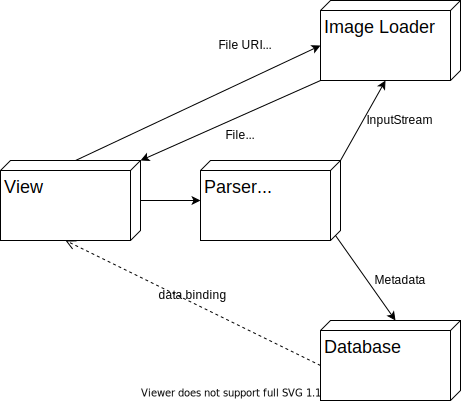
\includegraphics{../images/overall_architecture.svg}
\caption{overall architecture}
\end{figure}

Hình 1: Kiến trúc tổng quan của yacv

Ở Chương 2, trong phần về MVVM, yacv được giới thiệu là có sử dụng kiến
trúc này. Tuy nhiên, MVVM chỉ là một phần nhỏ của ứng dụng, chủ yếu liên
quan đến việc hiển thị dữ liệu nên chỉ có ý nghĩa khi xét đến các thành
phần trong module \textbf{View}.

yacv chỉ thiết kế cho \emph{một người dùng}, do đó có rất ít tương tác,
dẫn đến kiến trúc tối giản và rời rạc như trên. Các tiểu mục sau sẽ đi
sâu vào các module này.

\hypertarget{module-database}{%
\subsubsection{\texorpdfstring{4.1. Module Database
}{4.1. Module Database }}\label{module-database}}

Thông thường mục này được tách riêng ra, xếp vào mục \emph{Thiết kế cơ
sở dữ liệu}, ngang hàng với mục Thiết kế hướng đối tượng. Tuy nhiên,
yacv còn cần xử lí dữ liệu khác quan trọng không kém là dữ liệu ảnh. Do
không còn có vai trò trung tâm, duy nhất, phần cơ sở dữ liệu chỉ được
coi là một module trong thiết kế hướng đối tượng của ứng dụng.

yacv chọn SQLite vì đây là một cơ sở dữ liệu gọn nhẹ nhúng sẵn trong
Android. SQLite sử dụng mô hình quan hệ, do đó thiết kế bảng cần đảm bảo
được chuẩn hóa (normalization).

Do không cần quản lí người dùng, cơ sở dữ liệu của yacv chỉ dùng để
\emph{lưu thông tin metadata}, cho phép ứng dụng quét dữ liệu ít lần hơn
và tìm kiếm truyện. Theo như yêu cầu về metadata ở hai Phụ lục, và sau
khi chuẩn hóa, ta có lược đồ cơ sở dữ liệu như sau:

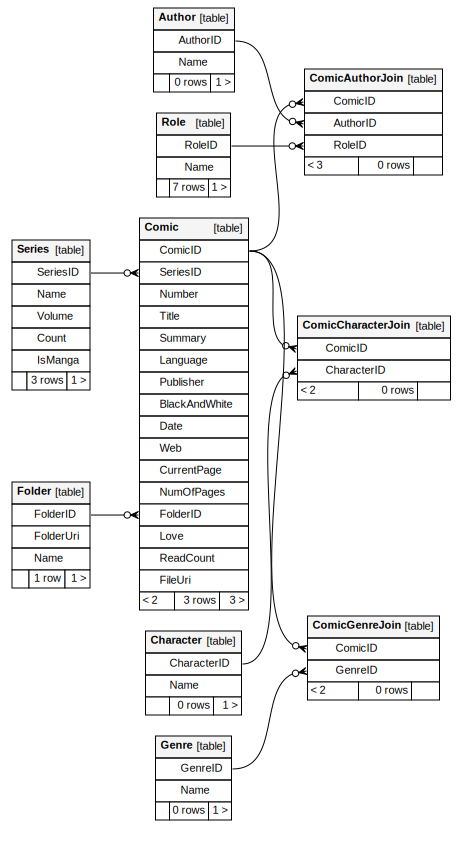
\includegraphics{../images/relationships.real.large.svg} Hình 2: Lược đồ
cơ sở dữ liệu của yacv

Các bảng thực thể gồm:

\begin{itemize}
\item
  \texttt{Comic}: lưu thông tin \emph{tập truyện lẻ}, là bảng trung tâm
\item
  \texttt{Series}: lưu thông tin \emph{bộ truyện}
\item
  \texttt{Author}: lưu tên tác giả
\item
  \texttt{Role}: lưu vai trò của tác giả trong một tập truyện
\item
  \texttt{Character}: lưu tên nhân vật
\item
  \texttt{Genre}: lưu tên thể loại truyện
\end{itemize}

Một hạn chế quan trọng của các bảng \texttt{Character} và
\texttt{Author} là chúng chỉ lưu thông tin tên, và chỉ phân biệt với
nhau bằng tên. Nếu có hai tác giả/nhân vật trùng tên, yacv không thể
phát hiện và hiển thị riêng.

Xét bảng trung tâm \texttt{Comic}. Bảng này có một số trường không phải
metadata mà dùng để lưu thông tin của riêng ứng dụng, gồm:

\begin{itemize}
\item
  \texttt{CurrentPage}: lưu trang đang đọc
\item
  \texttt{Love}: lưu trạng thái Yêu thích
\item
  \texttt{ReadCount}: lưu số lần đọc
\end{itemize}

Trong lược đồ, có nhiều trường nhìn qua không cần thiết nhưng thực tế có
ích, do thư viện SAF đã mô tả ở Chương 2:

\begin{itemize}
\item
  Trường \texttt{FileUri} trong \texttt{Comic}: Lưu đường dẫn của tệp
  truyện ở dạng URI.
\item
  Trường \texttt{FolderUri} trong \texttt{Folder}: Lưu đường dẫn của thư
  mục ở dạng URI.
\item
  Trường \texttt{Name} trong \texttt{Folder}: Tên thư mục. Thông thường
  nếu có đường dẫn, có thể tìm ra tên thư mục rất nhanh, tuy nhiên cũng
  do SAF mà việc này trở nên khó khăn, nên cần lưu riêng trường này.
\end{itemize}

Các trường URI đều cần có ràng buộc \texttt{UNIQUE}, do mỗi URI trỏ đích
danh đến một đối tượng.

Ta xem xét đến các bảng nối:

\begin{itemize}
\item
  \texttt{ComicCharacterJoin}:

  \begin{itemize}
    \item
    Mỗi tập truyện có thể có nhiều nhân vật và ngược lại, do đó
    \texttt{Comic} và \texttt{Character} có quan hệ Nhiều - Nhiều.
  \item
    Chú ý rằng các nhân vật có quan hệ với tập truyện chứ không phải bộ
    truyện, vì có nhân vật phụ (không xuất hiện trong mọi tập truyện).
  \end{itemize}
\item
  \texttt{ComicAuthorJoin}:

  \begin{itemize}
    \item
    Mỗi tập truyện có thể có nhiều tác giả và ngược lại, do đó
    \texttt{Comic} và \texttt{Author} có quan hệ Nhiều - Nhiều.
  \item
    Chú ý rằng các tác giả có quan hệ với tập truyện chứ không phải bộ
    truyện, vì mô hình xuất bản nhiều truyện tranh là nhà xuất bản sở
    hữu nhân vật và thuê người viết.
  \item
    Đồng thời, một tác giả có thể giữ vai trò khác nhau trong các bộ
    truyện khác nhau, do đó bảng này còn nối với bảng \texttt{Role}.
  \end{itemize}
\item
  \texttt{ComicGenreJoin}: Mỗi tập truyện có thể có nhiều thể loại khác
  nhau và ngược lại, do đó \texttt{Comic} và \texttt{Genre} có quan hệ
  Nhiều - Nhiều.
\end{itemize}

Do dùng Room, mỗi bảng ứng với một lớp. Các truy vấn với bảng cần đóng
gói dữ liệu vào các lớp này, trước khi gửi đến hoặc nhận về từ
\emph{DAO} (Data Access Object). Mỗi câu lệnh lại được chuyển thành một
hàm trong DAO.

\hypertarget{module-view-a-namep4.2-view-module}{%
\subsubsection{4.2. Module View \textless a
name="P4.2-view-module>}\label{module-view-a-namep4.2-view-module}}

Phần này tập trung vào các Màn hình, và phân tích chúng theo hướng MVVM.

Trong phần này có dùng nhiều biểu đồ tuần tự (sequence diagram) để minh
họa tương tác của ba thành phần MVVM (cùng với một số thành phần liên
quan) trong các ca sử dụng. Có một số điểm chung về các biểu đồ này:

\begin{itemize}
\item
  Trừ khi cần thiết, thành phần View sẽ được lược bỏ cho ngắn gọn.
\item
  Đường thẳng nét đứt thể hiện tính năng data binding (tự động cập nhật
  View), và thường trỏ về ViewModel. Đáng ra, mũi tên này phải trỏ về
  View, nhưng do View bị ẩn đi, nên nó trỏ về ViewModel. Mặc dù không
  được đề cập đến trong phần giới thiệu về MVVM, đây thực ra là một chi
  tiết đúng về mặt kĩ thuật: ViewModel hoàn toàn đọc được luồng dữ liệu
  gửi đến View (hoặc ít nhất là đúng trong cách viết ứng dụng Android
  thông thường).
\end{itemize}

Các biểu đồ trạng thái cũng có một số chi tiết chung:

\begin{itemize}
\item
  Trừ khi nêu rõ, mọi trạng thái đều có thể là trạng thái bắt đầu (trạng
  thái khi mở ứng dụng) hoặc kết thúc (khi đóng ứng dụng).
\item
  Mũi tên chuyển trạng thái tương ứng với \emph{tương tác của người
  dùng}, do vậy thường được ánh xạ đến một phương thức trong View.
\item
  Kí hiệu hình tròn đen chỉ dùng để tả trạng thái đầu \emph{khi lần đầu
  dùng} yacv.
\end{itemize}

Biểu đồ lớp thường có một phương thức chung là ``Get InputStream from
ID''. Cách truy cập để lấy \texttt{InputStream} của ảnh từ
\texttt{ComicID} có thể tham khảo từ Màn hình Đọc truyện.

\hypertarget{nguux1ed3n-dux1eef-liux1ec7u---repository---dao---comicparser}{%
\paragraph{\texorpdfstring{4.2.1. Nguồn dữ liệu - Repository - DAO -
ComicParser
}{4.2.1. Nguồn dữ liệu - Repository - DAO - ComicParser }}\label{nguux1ed3n-dux1eef-liux1ec7u---repository---dao---comicparser}}

Như đã đề cập ở Chương 2, yacv sử dụng Kiến trúc Google khuyên dùng, vốn
dựa trên MVVM. Phần này nêu rõ hơn cách triển khai MVVM của yacv trong
phần nguồn dữ liệu (Model/Repository).

Dựa vào Hình 9, ta thiết kế được 3 nguồn dữ liệu (model) sau:

\begin{longtable}[]{@{}lll@{}}
\toprule
& Thành phần tương đương & Mục đích \\
\midrule
\endhead
ComicParser & Remote Data Source & Quét tệp để lấy metadata cập nhật
nhất \\
DAO & Model & Lấy metadata từ cơ sở dữ liệu để tránh quét đi quét lại \\
Repository & Repository & Tổng hợp hai nguồn trên \\
\bottomrule
\end{longtable}

Bảng 3: Ba nguồn dữ liệu tương đương với Hình 9

Cụ thể hơn, \emph{ComicParser} là bộ quét metadata tệp truyện (thuộc
module Parser \& Scanner, sẽ được mô tả sau). Lớp này nhận vào URI rồi
trả về metadata của tệp truyện tương ứng dưới dạng đối tượng
\texttt{Comic}.

Khi cần đọc dữ liệu metadata từ tệp truyện, ba thành phần này tương tác
như sau:

\begin{figure}
\centering
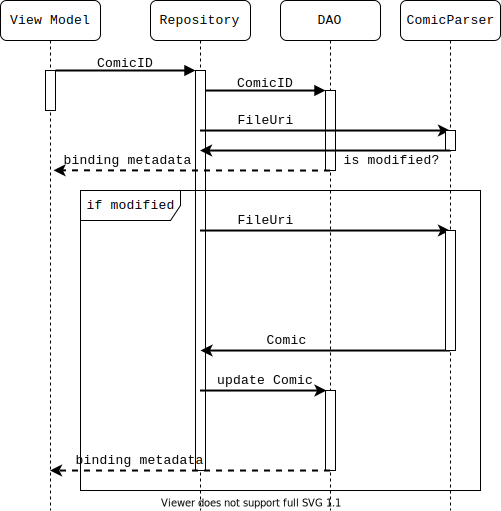
\includegraphics{../images/repo_mvvm_sequence.svg}
\caption{mvvm repo}
\end{figure}

Hình 11: Tương tác của ba nguồn dữ liệu, mũi tên gạch đứt thể hiện tính
năng data binding

Mấu chốt ở đây là ComicParser dù có dữ liệu chính xác (trong trường hợp
một ứng dụng khác sửa metadata tệp truyện) nhưng tốc độ rất chậm, còn cơ
sở dữ liệu không chính xác nhưng rất nhanh, do đó \emph{cơ sở dữ liệu
làm bộ đệm cho parser}.

Repository làm nhiệm vụ gọi cả hai nguồn dữ liệu trên và cập nhật cơ sở
dữ liệu (nếu cần) thay cho View/ViewModel. Hiện tại, Repository có thể
không làm được nhiều, tuy nhiên nó giúp ích cho \emph{khả năng mở rộng}
của ứng dụng. Ví dụ, trong tương lai yacv có thể liên kết với một bên
thứ ba cung cấp metadata cho truyện, khi đó để tích hợp API thì chỉ cần
sửa phần Repository.

Cũng cần chú ý rằng việc đọc metadata từ tệp tin không phải là yêu cầu
của mọi màn hình (cụ thể chỉ Màn hình Metadata cần), do đó trong đa số
các ca sử dụng, \emph{DAO đóng vai trò Model}, thay cho Repository.
Tương tác trong Hình 11 vẫn được duy trì, tuy không có cả Repository lẫn
ComicParser.

\hypertarget{muxe0n-huxecnh-quyux1ec1n-ux111ux1ecdc}{%
\subparagraph{\texorpdfstring{4.2.2. Màn hình Quyền đọc
}{4.2.2. Màn hình Quyền đọc }}\label{muxe0n-huxecnh-quyux1ec1n-ux111ux1ecdc}}

Do sự phức tạp trong việc xin quyền của Android, một màn hình riêng để
xin quyền đọc dữ liệu được tách ra khỏi Màn hình Thư viện, gọi là
\emph{Màn hình Quyền đọc}. Màn hình này sẽ là \emph{màn hình đầu tiên}
hiển thị khi dùng ứng dụng.

\begin{itemize}
\item
  Nếu có quyền đọc: chuyển ngay sang Màn hình Thư viện
\item
  Nếu không: nêu lí do cần quyền, gợi ý người dùng cấp quyền
\end{itemize}

Hình 12 mô tả trạng thái cấp quyền đọc của yacv (cũng như mọi quyền của
một ứng dụng Android cơ bản nói chung).

\begin{figure}
\centering
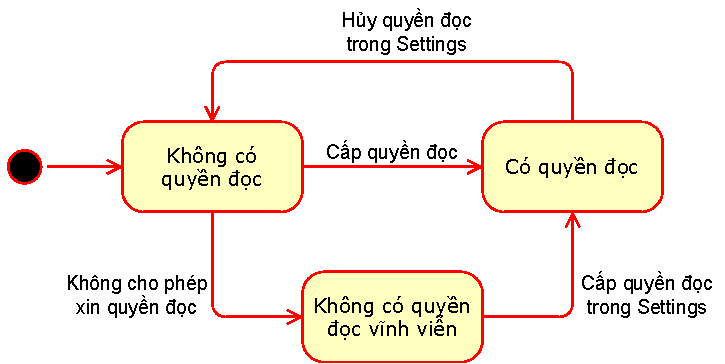
\includegraphics{../images/read_permission_state.svg}
\caption{permission state}
\end{figure}

Hình 12: Trạng thái cấp quyền của yacv

Dựa theo Hình 12, ta có biểu đồ lớp của ViewModel và View như sau:

\begin{figure}
\centering
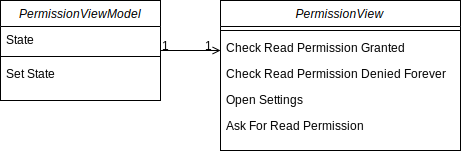
\includegraphics{../images/read_permission_mvvm_class.svg}
\caption{permission mvvm}
\end{figure}

Hình 12: Biểu đồ lớp của Màn hình Quyền đọc

\hypertarget{muxe0n-huxecnh-thux1b0-viux1ec7n}{%
\subparagraph{\texorpdfstring{4.2.3. Màn hình Thư viện
}{4.2.3. Màn hình Thư viện }}\label{muxe0n-huxecnh-thux1b0-viux1ec7n}}

Màn hình Thư viện là một trong hai màn hình của ca sử dụng Duyệt truyện,
bên cạnh Màn hình Thư mục.

Như đã phân tích ở \protect\hyperlink{P3.3.2-show-library}{mục 3.3.2},
Màn hình Thư viện cần hiển thị cả lỗi và gợi ý, bên cạnh việc hiển thị
danh sách thư mục và chọn thư mục gốc. Do đó, phần này chia ra làm hai
phần con tương ứng.

4.2.3.1. Chọn thư mục gốc và hiển thị danh sách thư mục

Để chọn thư mục gốc, người dùng ấn nút Đổi thư mục gốc để kích hoạt hộp
thoại Chọn thư mục (picker), rồi chọn một thư mục trong đó. Luồng chạy
của yacv như sau (trường hợp ngoại lệ sẽ được nêu trong phần kế tiếp):

\begin{figure}
\centering
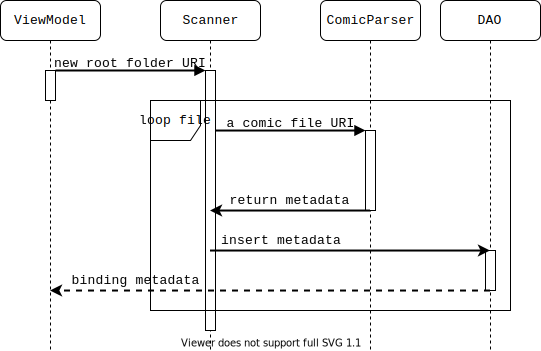
\includegraphics{../images/scanning_sequence.svg}
\caption{scanning}
\end{figure}

Hình 13: Quét tệp truyện khi thay đổi thư mục gốc và hiển thị

\emph{Scanner} là đối tượng để quét dữ liệu. Scanner nhận vào URI của
thư mục gốc, rồi lặp qua từng tệp con, cháu,\ldots{} Nếu đó là tệp
truyện, nó gọi Parser để lấy metadata, rồi lưu vào cơ sở dữ liệu qua
DAO.

Quá trình quét tệp này giống như duyệt cây, do đó có hai cách cơ bản:

\begin{itemize}
\item
  Duyệt theo độ sâu (depth-first search, gọi tắt là DFS)
\item
  Duyệt theo độ rộng (breadth-first search, gọi tắt là BFS)
\end{itemize}

Trong trường hợp cụ thể này, DFS được chọn. Lý do cho lựa chọn này là
DFS có thể phát hiện \emph{thư mục} nhanh hơn nhiều so với BFS. Mỗi khi
gặp thư mục, DFS xử lí (đi xuống các thư mục con) ngay, thay vì thêm vào
hàng đợi. Do phát hiện được thư mục nhanh hơn BFS, Màn hình Thư viện,
vốn hiển thị danh sách các \emph{thư mục}, cũng hiển thị sớm hơn. Dù
thời gian quét tổng thể không thay đổi, người dùng được thấy thư mục sớm
hơn giúp tạo cảm giác ứng dụng khá nhanh.

4.2.3.2. Ngoại lệ trong Màn hình Thư viện

Ngoại lệ ở đây chỉ cả trường hợp không tìm thấy thư mục, lẫn trường hợp
không quét được thư mục vì các lí do đã nêu trong
\protect\hyperlink{P3.3.1-scan}{mục 3.1}. Khi này, ứng dụng hiển thị một
hàng chữ để gợi ý về việc nên làm.

Hình sau là biểu đồ trạng thái, cũng là mô tả về nội dung gợi ý. Riêng
trạng thái ``Có truyện'' là trạng thái hiển thị danh sách thư mục trong
luồng cơ bản đã nêu trên, tức thư mục được hiển thị đầy đủ thay vì chỉ
hiện thông báo lỗi.

\begin{figure}
\centering
\includegraphics{../images/library_state.svg}
\caption{library state}
\end{figure}

Hình 14: Trạng thái của Màn hình Thư viện

Tổng hợp lại, ta có biểu đồ lớp của Màn hình Thư viện như sau:

\begin{figure}
\centering
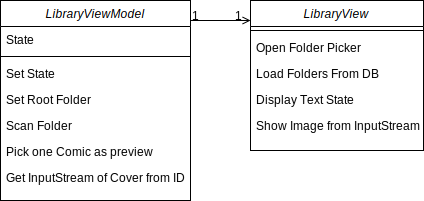
\includegraphics{../images/library_mvvm_class.svg}
\caption{library mvvm}
\end{figure}

Hình 15: Biểu đồ lớp của Màn hình Thư viện

Nhắc lại, cách truy cập để lấy \texttt{InputStream} của ảnh từ
\texttt{ComicID} có thể tham khảo từ Màn hình Đọc truyện.

\hypertarget{muxe0n-huxecnh-thux1b0-mux1ee5c}{%
\subparagraph{\texorpdfstring{4.2.4. Màn hình Thư mục
}{4.2.4. Màn hình Thư mục }}\label{muxe0n-huxecnh-thux1b0-mux1ee5c}}

Màn hình Thư mục là một trong hai màn hình của ca sử dụng Duyệt truyện,
bên cạnh Màn hình Thư viện.

Trong khi phân tích yêu cầu, ta đã phân tích được rằng màn hình hiển thị
danh sách truyện - một phần trong
\protect\hyperlink{P3.3.5-search-comic}{ca sử dụng tìm kiếm} - phải có
giao diện giống Màn hình Thư mục, vì đều hiển thị danh sách truyện. Do
đó, hai màn hình này được gộp lại, gọi chung là \emph{Màn hình Danh sách
truyện}, và sẽ được mô tả sau.

\hypertarget{muxe0n-huxecnh-ux111ux1ecdc-truyux1ec7n}{%
\subparagraph{\texorpdfstring{4.2.5. Màn hình Đọc truyện
}{4.2.5. Màn hình Đọc truyện }}\label{muxe0n-huxecnh-ux111ux1ecdc-truyux1ec7n}}

Để hiển thị các trang truyện, Màn hình Đọc truyện cần nhận
\texttt{ComicID} (hoặc một đối tượng \texttt{Comic} hoàn chỉnh, tuy
nhiên cốt yếu vẫn là thông tin \texttt{ComicID}) của một tệp truyện, sau
đó đưa cho \texttt{ComicParser} để lấy luồng đọc cho từng trang truyện.
Biểu đồ luồng của màn hình này là như sau:

\begin{figure}
\centering
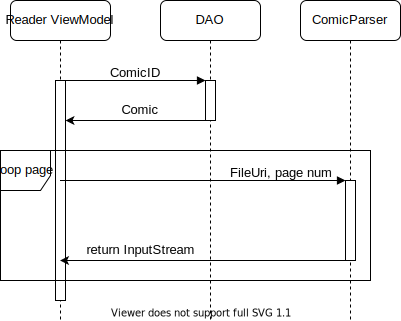
\includegraphics{../images/reader_sequence.svg}
\caption{reader sequence}
\end{figure}

Hình 16: Biểu đồ tuần tự của Màn hình Đọc truyện

Ta cũng có biểu đồ lớp tương ứng:

\begin{figure}
\centering
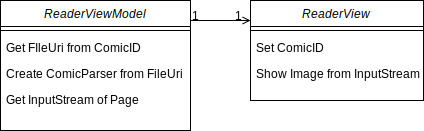
\includegraphics{../images/reader_mvvm_class.svg}
\caption{reader class}
\end{figure}

Hình 17: Biểu đồ lớp của Màn hình Đọc truyện

\hypertarget{muxe0n-huxecnh-metadata}{%
\subparagraph{\texorpdfstring{4.2.6. Màn hình Metadata
}{4.2.6. Màn hình Metadata }}\label{muxe0n-huxecnh-metadata}}

Màn hình Metadata tuân theo biểu đồ tuần tự đã nêu ở Hình 11. Biểu đồ
lớp tương ứng của màn hình này như sau:

\begin{figure}
\centering
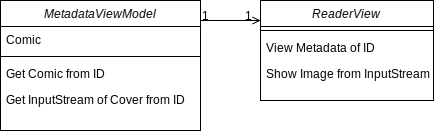
\includegraphics{../images/metadata_mvvm_class.svg}
\caption{metadata mvvm}
\end{figure}

Hình 18: Biểu đồ lớp của Màn hình Metadata

\hypertarget{muxe0n-huxecnh-tuxecm-kiux1ebfm}{%
\subparagraph{\texorpdfstring{4.2.7. Màn hình Tìm kiếm
}{4.2.7. Màn hình Tìm kiếm }}\label{muxe0n-huxecnh-tuxecm-kiux1ebfm}}

Màn hình Tìm kiếm là hai trong ba màn hình của
\protect\hyperlink{P3.3.5-search-comic}{ca sử dụng tìm kiếm truyện}, bên
cạnh Màn hình Danh sách truyện (là tổng quát hóa của Màn hình Thư mục,
đã nhắc ở trên). Màn hình Danh sách truyện sẽ được thiết kế ở ngay mục
sau, còn mục này tập trung vào Màn hình Tìm kiếm.

Không khó để thấy thực ra Màn hình Tìm kiếm Tổng quan và Màn hình Tìm
kiếm Chi tiết thực ra là một màn hình, về mặt thị giác:

\begin{itemize}
\item
  Điểm giống:

  \begin{itemize}
    \item
    Cả hai cùng hiển thị danh sách.
  \item
    Các phần tử cùng loại trong hai màn hình có cách hiển thị giống
    nhau, chuyển đến các màn hình giống nhau.
  \end{itemize}
\item
  Điểm khác: Danh sách trong Màn hình Tìm kiếm Tổng quan có \emph{thêm}:

  \begin{itemize}
    \item
    Hiển thị bìa với một số kết quả
  \item
    Có thanh ngăn cách
  \item
    Có nút ``Xem thêm''
  \end{itemize}
\end{itemize}

Do vậy, nếu thiết kế phù hợp, hoàn toàn có thể gộp hai màn hình này. Tôi
quyết định gộp lại, và gọi chung là Màn hình Tìm kiếm. Thiết kế sau giúp
thỏa mãn việc gộp hai màn hình:

\begin{itemize}
\item
  Màn hình nhận vào một tham số chứa \emph{câu truy vấn}. Tham số này
  thuộc một trong hai kiểu:

  \begin{itemize}
    \item
    \texttt{QuerySingleType}: chứa câu truy vấn và \emph{một} bảng để
    tìm kiếm
  \item
    \texttt{QueryMultipleTypes}: chứa câu truy vấn và một \emph{danh
    sách} bảng để tìm kiếm
  \end{itemize}

  ``Bảng để tìm kiếm'' thực ra là một số quy định trước, ví dụ nếu là số
  \texttt{0} thì bảng được tìm là \texttt{Comic},\ldots{}
\item
  ViewModel tìm kiếm dựa vào tham số truy vấn

  \begin{itemize}
    \item
    Nếu tham số là \texttt{QuerySingleType}: truy vấn và hiển thị kết
    quả như thông thường
  \item
    Nếu tham số là \texttt{QueryMultipleTypes}: truy vấn các bảng, gộp
    kết quả lại và thêm kiểu kết quả đặc biệt là \emph{Placeholder} và
    \emph{SeeMore} vào vị trí phù hợp để hiển thị lần lượt nhóm kết quả
    và nút ``Xem thêm''
  \end{itemize}
\item
  Các kết quả, bao gồm hai dạng kết quả đặc biệt ở trên, cài đặt chung
  giao diện \texttt{Metadata}, để có thể được gộp thành một danh sách
\end{itemize}

Nói ngắn gọn, hai màn hình cùng hiển thị một danh sách, danh sách này có
một số phần tử đánh dấu đặc biệt. Ta dùng lại ví dụ về truy vấn
\texttt{Watchmen} ở Chương 3 để minh họa:

\begin{itemize}
\item
  Truy vấn \texttt{QueryMultipleTypes} được gửi đến Màn hình Tìm kiếm.
  Câu truy vấn là \texttt{Watchmen}, các bảng cần tìm là mọi bảng.
\item
  ViewModel tìm \texttt{Watchmen} trong mọi bảng, tìm được:

  \begin{itemize}
    \item
    3 tệp truyện trong bảng \texttt{Comic}
  \item
    2 bộ truyện trong bảng \texttt{Series}
  \end{itemize}
\item
  Màn hình hiển thị:

  \begin{enumerate}
  \def\labelenumi{\arabic{enumi}.}
    \item
    Dòng \texttt{Truyện}, rồi 3 tệp truyện (cùng với ảnh bìa)
  \item
    Dòng \texttt{Bộ\ truyện}, 1 bộ truyện, rồi dòng \texttt{Xem\ thêm}
  \end{enumerate}
\item
  Khi ấn vào:

  \begin{itemize}
    \item
    Một trong ba tệp truyện: Đưa đến Màn hình Đọc truyện tương ứng.
  \item
    Một bộ truyện: Chuyển đến Màn hình Danh sách truyện, chứa các truyện
    trong bộ đó.
  \item
    Nút \texttt{Xem\ thêm}: Chuyển đến Màn hình Tìm kiếm, lần này tham
    số là một \texttt{QuerySingleType}, với câu truy vấn là
    \texttt{Watchmen}, còn bảng để tìm là \texttt{Series}. Hai bộ truyện
    kết quả được hiển thị đầy đủ. Chọn một bộ truyện lúc này giống với
    chọn bộ truyện ở trên (sang Màn hình Danh sách truyện).
  \end{itemize}
\end{itemize}

Biểu đồ lớp của các đối tượng liên quan như sau:

\begin{longtable}[]{@{}ll@{}}
\toprule
Hình 19a: Biểu đồ lớp \texttt{Query} & Hình 19b: Biểu đồ lớp
\texttt{Metadata} \\
\midrule
\endhead
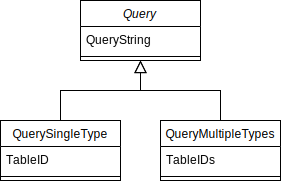
\includegraphics{../images/query_class.svg} &
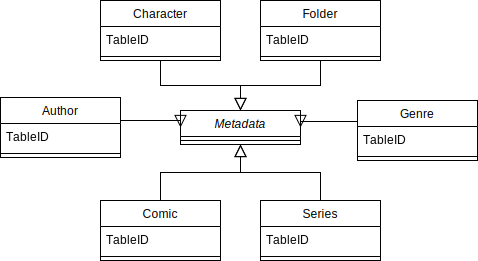
\includegraphics{../images/metadata_class.svg} \\
\bottomrule
\end{longtable}

Hình 19: Biểu đồ các lớp liên quan đến Màn hình Tìm kiếm

Biểu đồ lớp của bản thân Màn hình Tìm kiếm như sau:

\begin{figure}
\centering
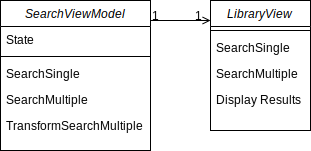
\includegraphics{../images/search_mvvm_class.svg}
\caption{search mvvm}
\end{figure}

Hình 20: Biểu đồ lớp của Màn hình Tìm kiếm

Do mỗi DAO trả kết quả của bảng tương ứng về ở dạng danh sách, nên khi
dùng \texttt{QueryMultipleTypes}, các danh sách kết quả lẻ này tổng hợp,
và thêm hai kiểu kết quả đặc biệt. Hàm
\texttt{TransformSearchMultiple()} là để ``làm phẳng'' mảng kết quả hai
chiều như trên.

Chương 5 sẽ có một ví dụ về việc tìm kiếm, cho thấy yacv có thể hiển thị
từ từ kết quả tìm kiếm theo quá trình tìm như thế nào.

\hypertarget{muxe0n-huxecnh-danh-suxe1ch-truyux1ec7n}{%
\subparagraph{\texorpdfstring{4.2.8. Màn hình Danh sách truyện
}{4.2.8. Màn hình Danh sách truyện }}\label{muxe0n-huxecnh-danh-suxe1ch-truyux1ec7n}}

Màn hình này là màn hình thứ ba trong chuỗi các màn hình liên quan đến
ca sử dụng tìm kiếm, đồng thời đóng vai trò của Màn hình Thư mục (do là
phiên bản tổng quát hơn của nó).

Màn hình này nhận vào một tham số kiểu \texttt{Metadata} thay vì một
\texttt{Query}, và trả về danh sách các \emph{tệp truyện} -
\texttt{Comic} - có liên kết với tham số đầu vào.

Biểu đồ lớp của Màn hình Danh sách truyện như sau:

\begin{figure}
\centering
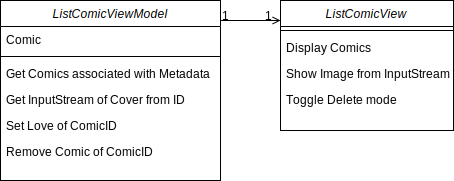
\includegraphics{../images/list_comics_mvvm_class.svg}
\caption{list comic mvvm}
\end{figure}

Hình 21: Biểu đồ lớp của Màn hình Danh sách truyện

\hypertarget{module-parser-scanner-a-namep4.3-parser-scanner-module}{%
\subsubsection{4.3. Module Parser \& Scanner \textless a
name="P4.3-parser-scanner-module>}\label{module-parser-scanner-a-namep4.3-parser-scanner-module}}

Điểm chung để gom hai thành phần này vào một module là chúng làm việc
trực tiếp với tệp truyện nén.

\hypertarget{comicparser-a-namep4.3.1-comic-parser}{%
\paragraph{\texorpdfstring{4.3.1. \texttt{ComicParser} \textless a
name="P4.3.1-comic-parser>}{4.3.1. ComicParser \textless a name="P4.3.1-comic-parser>}}\label{comicparser-a-namep4.3.1-comic-parser}}

\texttt{ComicParser} là một trong các thành phần trung tâm của yacv. Lớp
này nhận vào URI trỏ đến một tệp truyện, và đọc nội dung tệp truyện đó
ra. Cần gọi đủ tên là \texttt{ComicParser}, vì phải phân biệt với hai
parser (bộ đọc/giải mã) khác nhưng tích hợp trong nó:

\begin{longtable}[]{@{}
  >{\raggedright\arraybackslash}p{(\columnwidth - 4\tabcolsep) * \real{0.18}}
  >{\raggedright\arraybackslash}p{(\columnwidth - 4\tabcolsep) * \real{0.40}}
  >{\raggedright\arraybackslash}p{(\columnwidth - 4\tabcolsep) * \real{0.42}}@{}}
\toprule
& Parser cho tệp nén & Parser cho metadata \\
\midrule
\endhead
Đầu vào & Tệp nén & Tệp metadata \\
Đầu ra & Các tệp con hoặc tương đương (ví dụ như luồng đọc đến tệp con)
& Đối tượng \texttt{Comic} \\
\bottomrule
\end{longtable}

Bảng 4: Hai kiểu parser trong \texttt{ComicParser}

\texttt{ComicParser} được thiết kế theo kiểu ``lười'', có nghĩa là không
có thông tin nào được đọc ra cho đến khi thực sự cần. Lý do vẫn là vấn
đề về hiệu năng, vì gần như mọi thao tác đọc trong SAF - hệ thống đọc
ghi tệp của Android - đều rất chậm.

\hypertarget{parser-cho-tux1ec7p-nuxe9n}{%
\subparagraph{4.3.1.1. Parser cho tệp
nén}\label{parser-cho-tux1ec7p-nuxe9n}}

Parser cho tệp nén hiện gồm một giao diện và hai lớp

\begin{itemize}
\item
  \texttt{ArchiveParser}: giao diện chung cho mọi parser tệp nén
\item
  \texttt{CBZParser}: parser riêng cho tệp CBZ
\item
  \texttt{ArchiveParserFactory}: giúp khởi tạo các parser
\end{itemize}

\texttt{ArchiveParser} là một giao diện (interface), định nghĩa một số
phương thức chung mọi parser cho tệp nén đều phải có. Do hiện tại yacv
mới hỗ trợ định dạng CBZ, chỉ có lớp \texttt{CBZParser} cài đặt giao
diện này.

Trong \texttt{ArchiveParser}, có hai phương thức quan trọng:

\begin{itemize}
\item
  \texttt{getEntryOffsets()}: Phương thức này trả về một từ điển như
  sau:

  \begin{itemize}
    \item
    Khóa: tên tệp lẻ
  \item
    Giá trị: offset tệp lẻ, tức vị trí tệp lẻ trong tệp nén
  \end{itemize}
\item
  \texttt{readEntryAtOffset()}: Phương thức này nhận vào một offset, và
  trả về luồng đọc tương ứng với tệp lẻ ở offset đó bằng cách ``nhảy
  cóc'' đến đúng chỗ và đọc.
\end{itemize}

\texttt{ArchiveParserFactory} là một lớp theo mẫu thiết kế factory, nhận
vào URI của tệp truyện và trả về \texttt{ArchiveParser} để đọc loại tệp
truyện đó (ví dụ, nếu URI có đuôi CBZ thì trả về một đối tượng
\texttt{CBZParser}). Do \texttt{ArchiveParser} cần một số cài đặt khởi
tạo riêng, nên mới cần một lớp riêng để tạo parser. Chữ ``Factory'' thể
hiện lớp này sử dụng mẫu thiết kế factory.

\hypertarget{parser-cho-metadata}{%
\subparagraph{4.3.1.2. Parser cho metadata}\label{parser-cho-metadata}}

yacv hiện hỗ trợ định dạng ComicRack, được giới thiệu chi tiết trong Phụ
lục 2. Định dạng này là một tệp tin XML, do đó được đọc đơn giản bằng
các thư viện XML sẵn có.

Để mở rộng định dạng tệp đọc, có thể dùng mẫu thiết kế factory như đã
dùng với parser cho tệp. Theo cách này, các parser cần có hàm
\texttt{parse()} trả về một đối tượng \texttt{Comic} và nhận hai tham
số:

\begin{itemize}
\item
  Nội dung tệp metadata: ở dạng chuỗi thông thường
\item
  Tên tệp metadata: tên tệp giúp phân biệt các định dạng tệp với nhau
\end{itemize}

\hypertarget{cbzparser-a-namep4.3.2-cbzparser}{%
\paragraph{\texorpdfstring{4.3.2. \texttt{CBZParser} \textless a
name="P4.3.2-cbzparser>}{4.3.2. CBZParser \textless a name="P4.3.2-cbzparser>}}\label{cbzparser-a-namep4.3.2-cbzparser}}

\texttt{CBZParser} là lớp cài đặt giao diện \texttt{ArchiveParser}. Như
đã phân tích ở Chương 2, hệ thống đọc ghi tệp SAF của Android chỉ cho
phép đọc ghi tuần tự. Việc tạo ra mảng offset không đơn giản, do phần
mục lục của tệp ZIP nằm ở cuối, và có nhiều thao tác cần dò ngược từ
cuối lên.

Để giải quyết vấn đề danh sách offset, có hai cách đơn giản nhất:

\begin{itemize}
\item
  Chép toàn bộ tệp truyện vào phần bộ nhớ riêng của ứng dụng

  \begin{itemize}
  \item
    Ưu: Phần bộ nhớ này vẫn được dùng API File của Java, do đó có thể
    đọc ghi ngẫu nhiên, cho phép đọc mục lục rất nhanh.
  \item
    Nhược: Tệp truyện rất nặng (vài chục đến vài trăm MB) dẫn đến tốn cả
    dung lượng đĩa lẫn băng thông đọc/ghi. Ghi xóa liên tục cũng có hại
    cho bộ nhớ thể rắn của điện thoại.
  \end{itemize}
\item
  Đọc tệp ZIP ở chế độ đọc tuần tự

  \begin{itemize}
    \item
    Ưu: Dùng ngay được với cơ chế đọc qua \texttt{InputStream} của SAF
  \item
    Nhược: Do không có mục lục, dữ liệu phải được ``dò'' từ từ để đọc
    từng tệp lẻ một. Hậu quả là phương pháp này vừa tốn băng thông đọc,
    vừa tốn CPU để giải nén những tệp không cần thiết.
  \end{itemize}
\end{itemize}

\texttt{CBZParser} giải quyết vấn đề này bằng cách làm giả một luồng đọc
ngẫu nhiên, được miêu tả rõ hơn trong Chương 5. Cách làm đó có thể được
tóm tắt như sau:

\begin{itemize}
\item
  Hai phần đầu tệp nén được lưu đệm trong RAM, do là hai phần có nhiều
  truy cập nhất trong khi đọc mục lục
\item
  Các phần còn lại được đọc xuôi khi cần theo luồng nhập
  \texttt{InputStream}, nếu đọc ngược sẽ phải tạo mới luồng nhập
\end{itemize}

Kết quả là mục lục đọc được mà chỉ cần:

\begin{itemize}
\item
  Trung bình hai lần đọc tuần tự theo \texttt{InputStream}
\item
  Không phải ghi ra đĩa
\item
  Không phải giải nén những tệp không cần thiết
\end{itemize}

\hypertarget{tux1ed5ng-hux1ee3p-lux1ea1i-comicparser-a-namep4.3.3-comic-parser-revisited}{%
\paragraph{\texorpdfstring{4.3.3. Tổng hợp lại \texttt{ComicParser}
\textless a
name="P4.3.3-comic-parser-revisited>}{4.3.3. Tổng hợp lại ComicParser \textless a name="P4.3.3-comic-parser-revisited>}}\label{tux1ed5ng-hux1ee3p-lux1ea1i-comicparser-a-namep4.3.3-comic-parser-revisited}}

Tương tác trong một ca sử dụng hiển thị của \texttt{ComicParser} được mô
tả như sau:

\begin{figure}
\centering
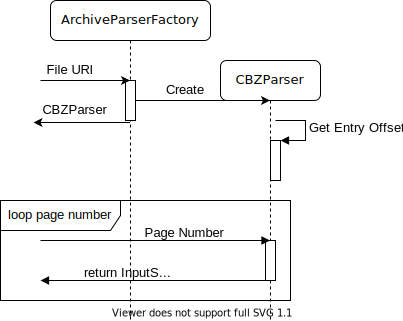
\includegraphics{../images/parser_sequence.svg}
\caption{parser sequence}
\end{figure}

Hình 22: \texttt{ComicParser} và các thành phần của nó

Ở đây cần làm rõ chi tiết về việc sắp xếp tệp theo tên. Không có quy
chuẩn cho tên trang truyện, tuy nhiên đa số các tệp truyện đặt tên theo
định dạng sau:

\begin{verbatim}
X-Men Vol 40 1.jpg
|     |      |
|     |      Trang truyện số
|     Số Volume, Number,...
Tên tệp truyện
\end{verbatim}

Vấn đề với định dạng này xuất hiện khi truyện có nhiều hơn 10 trang. Khi
sắp xếp tệp ảnh theo ABC, các trang sẽ có thứ tự như sau:

\begin{verbatim}
X-Men Vol 40 1.jpg
X-Men Vol 40 10.jpg
X-Men Vol 40 11.jpg
...
X-Men Vol 40 19.jpg
X-Men Vol 40 2.jpg
...
\end{verbatim}

Ta thấy ngay rằng thứ tự tệp ảnh bị đảo lộn. Để giải quyết vấn đề này,
cần viết hàm so sánh riêng cho tên tệp ảnh. Ý tưởng ở đây là gom những
kí tự số liên tiếp với nhau thành một ``kí tự'' rồi mới so sánh. Đoạn mã
giả sau trình bày thuật toán:

\begin{verbatim}
def compare(str1, str2):
    arrs = []

    for str in [str1, str2]:
        arrtmp = []
        acc = []

        for char in str:
            if is_number(char):
                acc.append(char)
            else:
                if len(acc) != 0:
                    acc = ''.join(acc)
                    acc = to_num(acc)
                    arrtmp.append(acc)
                    acc = 0
                arrtmp.append(to_codepoint(char))

    return compare_left_to_right(arrs[0], arrs[1])
\end{verbatim}

\hypertarget{scanner-a-namep4.3.4-scanner}{%
\paragraph{4.3.4. Scanner \textless a
name="P4.3.4-scanner>}\label{scanner-a-namep4.3.4-scanner}}

Đây là lớp phục vụ cho tính năng quét truyện trong yacv. Biểu đồ luồng
của ca sử dụng \emph{quét mới} là như sau:

\begin{figure}
\centering
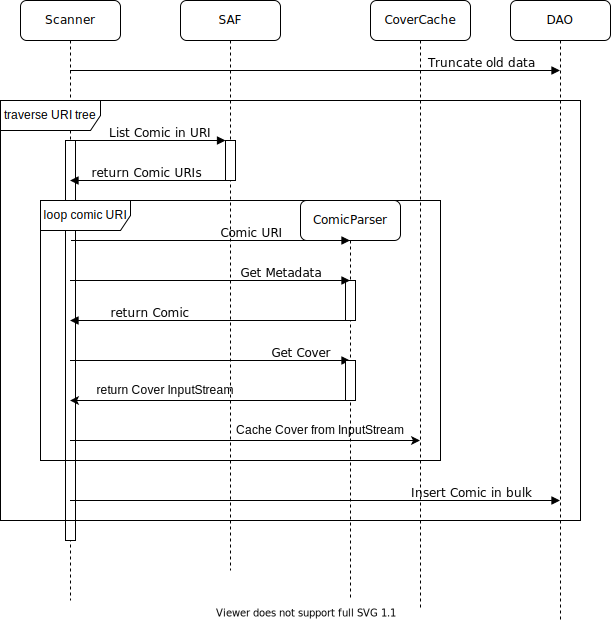
\includegraphics{../images/scan_new_sequence.svg}
\caption{new scan}
\end{figure}

Hình 23: Biểu đồ tuần tự của ca sử dụng quét mới tệp truyện

Một chi tiết mới trong biểu đồ này là lớp \texttt{ImageCache}, sẽ được
giới thiệu ở mục về cache ảnh.

Ca sử dụng quét lại cũng có thiết kế gần tương tự, trong đó bỏ bước xóa
dữ liệu, và thêm một bước quét cơ sở dữ liệu sau cùng để xóa truyện
không còn trong bộ nhớ. Việc cập nhật và thêm truyện mới được thực hiện
trong vòng lặp lớn bình thường.

\hypertarget{module-image-loader-a-namep4.4-image-loader-module}{%
\subsubsection{4.4. Module Image Loader \textless a
name="P4.4-image-loader-module>}\label{module-image-loader-a-namep4.4-image-loader-module}}

Module Image Loader chịu trách nhiệm trích xuất và lưu đệm (cache) tệp
ảnh. Module này gồm hai phần như sau:

\hypertarget{image-extractor-a-namep4.4.1-image-extractor}{%
\paragraph{4.4.1. Image Extractor \textless a
name="P4.4.1-image-extractor>}\label{image-extractor-a-namep4.4.1-image-extractor}}

Đây thực chất là một lớp đóng gói quanh \texttt{ComicParser}. Bản thân
chức năng trích xuất được thực hiện trong \texttt{ComicParser} (qua các
đối tượng \texttt{ArchiveParser}), tuy nhiên Image Extractor thực hiện
một số tối ưu giúp việc hiển thị ảnh nhanh chóng hơn.

Ở các mục trước, ta đã tệp lẻ trang truyện không được lưu theo thứ tự
đọc. Do đó, cần mục lục tệp nén để có thể nhảy cóc đến trang truyện theo
yêu cầu. Tuy nhiên, việc tải ảnh còn có thể tối ưu hơn nữa. Ta xét ví dụ
sau:

\begin{longtable}[]{@{}lll@{}}
\toprule
Thứ tự trong tệp nén & Tên tệp ảnh & Dung lượng \\
\midrule
\endhead
1 & \texttt{7.jpg} & 100KB \\
2 & \texttt{6.jpg} & 100KB \\
3 & \texttt{8.jpg} & 100KB \\
4 & \texttt{1.jpg} & 100KB \\
5 & \texttt{3.jpg} & 100KB \\
6 & \texttt{4.jpg} & 100KB \\
7 & \texttt{2.jpg} & 100KB \\
8 & \texttt{5.jpg} & 100KB \\
\bottomrule
\end{longtable}

Bảng 3: Danh sách các tệp ảnh trong một tệp truyện nén

Hiển nhiên, thứ tự ảnh cần xem là từ tệp \texttt{1.jpg} đến tệp
\texttt{8.jpg}. Ta xem xét và cải tiến các chiến lược tải ảnh qua các
tiểu mục tiếp theo.

\hypertarget{tux1ea3i-theo-yuxeau-cux1ea7u}{%
\subparagraph{4.4.1.1. Tải theo yêu
cầu}\label{tux1ea3i-theo-yuxeau-cux1ea7u}}

Ảnh được tải theo đúng yêu cầu ngay lúc đó. Quá trình đọc tệp tin như
sau:

\begin{itemize}
\item
  Đọc \texttt{1.jpg}: 100KB (bản thân ảnh) + 300KB (do trước khi đọc
  được \texttt{1.jpg} cần đi qua 3 ảnh \texttt{7.jpg}, \texttt{6.jpg},
  \texttt{8.jpg})
\item
  Đọc \texttt{2.jpg}: 100KB + 600KB
\item
  \ldots{}
\end{itemize}

Vậy để đọc hết truyện, cần đọc 4500KB. Chưa hết, luồng đọc phải được tạo
mới mỗi lần đọc (tức bằng số trang truyện), gây ra nhiều overhead. Lý do
là bản thân SAF là một Content Provider, do đó nó nằm ở một tiến trình
(process) riêng, và cần cơ chế liên lạc xuyên tiến trình (IPC) - vốn đắt
đỏ về mặt tính toán trên mọi hệ điều hành - để gọi.

Nguyên nhân của cả hai điểm yếu trên là việc không sử dụng lại luồng đọc
(mỗi luồng chỉ đọc một ảnh). Phương án tiếp theo cần xử lí được điểm yếu
này.

\hypertarget{tux1ed1i-thiux1ec3u-huxf3a-sux1ed1-luux1ed3ng-ux111ux1ecdc}{%
\subparagraph{4.4.1.2. Tối thiểu hóa số luồng
đọc}\label{tux1ed1i-thiux1ec3u-huxf3a-sux1ed1-luux1ed3ng-ux111ux1ecdc}}

Để giảm số luồng đọc, ta cần kiểm soát một vài luồng đọc, và phân mỗi
trang truyện cho một luồng đọc cụ thể. Để tối thiểu hóa số luồng đọc, ta
cần dùng thêm thuật toán \emph{chuỗi con tăng dài nhất} (longest
increasing subsequence). Thuật toán cuối cùng thể hiện bằng mã giả như
sau:

\begin{verbatim}
def minStream(pages):
    stream_count = 0
    map_idx_to_stream = []    # Từ điển ánh xạ số trang - số luồng

    while len(pages) != 0:
        # Dây trang tiến lên
        lis = longest_increasing_subsequence(pages)

        for page in lis:
            pages.remove_at(page)    # Bỏ trang trong dây khỏi danh sách
            map_idx_to_stream[page] = stream_count    # Gán số luồng hiện tại

        stream_count += 1

    return map_idx_to_stream
\end{verbatim}

Thuật toán nhận vào một mảng \texttt{pages} là \emph{thứ tự trong tệp
nén} của từng trang truyện. Thuật toán trả về một từ điển như sau:

\begin{itemize}
\item
  Khóa: trang truyện số (bắt đầu từ trang 1)
\item
  Giá trị: số luồng
\end{itemize}

Ta nhận thấy thuật toán hiển nhiên cho (xấp xỉ) số luồng ít nhất có thể,
vì mỗi lần chia trang cho các luồng, ta chọn một bộ trang tăng dần dài
nhất lúc đó.

Áp dụng vào ví dụ đang dùng, ta có:

\begin{itemize}
\item
  Luồng 0: đọc trang 1, 3, 4, 5
\item
  Luồng 1: đọc trang 7, 8
\item
  Luồng 2: đọc trang 6
\item
  Luồng 3: đọc trang 2
\end{itemize}

Vậy để đọc hết truyện, cần đọc 2000KB, và 4 lần tạo mới luồng đọc, khá
tốt so với phương pháp đầu. Tới đây chỉ cần một số chỉnh sửa nhỏ:

\begin{itemize}
\item
  Giới hạn số luồng đọc: Trường hợp xấu nhất là thứ tự trong tệp ZIP
  ngược với thứ tự đọc, do đó có nhiều luồng mà mỗi luồng chỉ phục vụ
  một trang truyện. yacv tránh điều này bằng cách giới hạn chỉ có 4
  luồng đọc cùng lúc. Những trang không ở trong phạm vi của các luồng
  này quay về cách đọc nhảy cóc thông thường, không dùng lại luồng đọc
  chờ sẵn.
\end{itemize}

\hypertarget{image-cache-a-namep4.4.2-image-cache}{%
\paragraph{4.4.2. Image Cache \textless a
name="P4.4.2-image-cache>}\label{image-cache-a-namep4.4.2-image-cache}}

Bản thân Image Cache \emph{không} phải là một đoạn mã, đối tượng, mà chỉ
là một thư mục. yacv có 2 loại/thư mục cache, cho hai trường hợp hiển
thị:

\begin{itemize}
\item
  Cache ảnh bìa
\item
  Cache trang truyện
\end{itemize}

Lý do cần đến hai bộ cache khác nhau là vì dung lượng lớn của truyện.
Các thư viện cache ảnh chọn mốc 100-200MB cho thư mục cache ảnh, đồng
thời dùng cố định phương pháp thay thế LRU (nếu cache đầy sẽ xóa ảnh lâu
nhất không được dùng). Khi đọc một bộ truyện dung lượng lớn hơn mốc này,
toàn bộ ảnh trong cache sẽ sớm bị thay thế bởi ảnh của trang truyện. Sau
khi đọc, quay về các màn hình, ảnh bìa dùng để hiển thị trong hai màn
hình duyệt truyện bị mất, gây suy giảm trải nghiệm người dùng. Do đó,
cần phải tách hai thư mục cache này ra để tránh ảnh hưởng đến cache
trang bìa.

\hypertarget{cache-trang-truyux1ec7n}{%
\subparagraph{4.4.2.1. Cache trang
truyện}\label{cache-trang-truyux1ec7n}}

Cache trang truyện có liên quan chặt chẽ đến Image Extractor. Khi đọc
một trang truyện, 3 trang kế và 1 trang trước được đảm bảo nằm sẵn trong
cache.

yacv chọn mốc 200MB để cache trang truyện. Android có thể xóa thư mục
cache này khi nào cần thêm dung lượng bộ nhớ.

Thư mục cache này được quản lí bởi thư viện hiển thị ảnh. Thư viện đó
nhận luồng đọc ảnh (từ Image Loader), ghi vào thư mục cache này, và xóa
ảnh để giải phóng dung lượng khi cần.

\hypertarget{cache-trang-buxeca}{%
\subparagraph{4.4.2.2. Cache trang bìa}\label{cache-trang-buxeca}}

Khác với cache trang truyện, cache trang bìa \emph{không} có liên quan
tới Image Loader. Thực ra ảnh bìa thì cũng được trích xuất bởi
\texttt{ComicParser}, tuy nhiên với mỗi tệp truyện chỉ cần trích ra một
ảnh bìa, do đó không cần cơ chế tái sử dụng luồng đọc phức tạp của Image
Loader.

Cache trang bìa lại gồm 2 thư mục cache:

\begin{enumerate}
\def\labelenumi{\arabic{enumi}.}
\item
  Cache ảnh hiển thị thực tế

  Cache ảnh được hiển thị bởi \texttt{ImageView}. Ảnh này là ảnh bìa đã
  được cắt (xem phần thiết kế màn hình duyệt truyện) và được thu phóng
  về chính xác kích cỡ khung nhìn. Dung lượng cache là 100MB.

  Cùng một bìa có hai kiểu hiển thị

  Thư mục cache này được quản lí bởi thư viện hiển thị ảnh. Thư viện đó
  nhận luồng đọc ảnh (từ \texttt{ComicParser}), ghi vào thư mục cache
  này, và xóa ảnh để giải phóng dung lượng khi cần.
\item
  Cache ảnh bìa thu nhỏ

  Cache ảnh bìa thu nhỏ, khoảng 50KB mỗi ảnh, chưa bị cắt. Dung lượng
  cache là 10MB.
\end{enumerate}

Lí do riêng phần bìa cần hai thư mục cache là vì cache ảnh hiển thị thực
tế, giống với cache trang truyện, có thể bị xóa bất cứ lúc nào. Do đó
cần có một cache rất nhỏ gọn, nằm ở thư mục riêng mà Android không xóa
được, chứa ảnh bìa chất lượng thấp, để khi ảnh bìa bị xóa vẫn có một bản
bìa nhỏ để hiển thị trong khi chờ ảnh bìa chất lượng cao, có cắt cúp phù
hợp được sinh lại.

Trong Hình 23, có một lớp \texttt{ImageCache} nhận \texttt{InputStream}
của ảnh bìa và cache ảnh, đó chính là lớp quản lí và sinh ảnh bìa thu
nhỏ.

\begin{center}\rule{0.5\linewidth}{0.5pt}\end{center}

\hypertarget{chux1b0ux1a1ng-5-lux1eadp-truxecnh-kiux1ec3m-thux1eed}{%
\subsection{\texorpdfstring{5. Chương 5: Lập trình \& Kiểm thử
}{5. Chương 5: Lập trình \& Kiểm thử }}\label{chux1b0ux1a1ng-5-lux1eadp-truxecnh-kiux1ec3m-thux1eed}}

Chương này nêu một số đoạn mã trong quá trình lập trình và kiểm thử,
cùng với ảnh chụp màn hình của kết quả cuối cùng.

\hypertarget{lux1eadp-truxecnh}{%
\subsubsection{\texorpdfstring{5.1. Lập trình
}{5.1. Lập trình }}\label{lux1eadp-truxecnh}}

\hypertarget{coroutine-1}{%
\paragraph{5.1.1. Coroutine}\label{coroutine-1}}

Về mặt lập trình, trong quá trình viết ứng dụng, một trong các khó khăn
chủ yếu là tăng tốc ứng dụng bằng coroutine. Sau đây trình bày một trong
những đoạn mã dùng coroutine trong ca sử dụng tìm kiếm, có sử dụng cả
LiveData:

\begin{Shaded}
\begin{Highlighting}[]
\NormalTok{suspend }\KeywordTok{fun} \FunctionTok{search}\OperatorTok{(}\VariableTok{query}\OperatorTok{:} \DataTypeTok{QueryMultipleTypes}\OperatorTok{,} \VariableTok{limit}\OperatorTok{:} \DataTypeTok{Int}\OperatorTok{):}
        \DataTypeTok{LiveData}\OperatorTok{<}\DataTypeTok{List}\OperatorTok{<}\DataTypeTok{List}\OperatorTok{<}\DataTypeTok{Metadata}\OperatorTok{>>>} \OperatorTok{=}\NormalTok{ liveData}\OperatorTok{(}\NormalTok{timeoutInMs }\OperatorTok{=} \DecValTok{3000}\OperatorTok{)} \OperatorTok{\{}
    \KeywordTok{val} \VariableTok{results2D} \OperatorTok{=}\NormalTok{ mutableListOf}\OperatorTok{<}\NormalTok{List}\OperatorTok{<}\NormalTok{Metadata}\OperatorTok{>>()}
    \KeywordTok{val} \VariableTok{latch} \OperatorTok{=}\NormalTok{ CountDownLatch}\OperatorTok{(}\NormalTok{daos}\OperatorTok{.}\NormalTok{size}\OperatorTok{)}

\NormalTok{    withContext}\OperatorTok{(}\NormalTok{Dispatchers}\OperatorTok{.}\NormalTok{IO}\OperatorTok{)} \OperatorTok{\{}
\NormalTok{        daos}\OperatorTok{.}\NormalTok{parallelForEach }\OperatorTok{\{}\NormalTok{ dao }\OperatorTok{{-}>}
            \KeywordTok{val} \VariableTok{results} \OperatorTok{=}\NormalTok{ dao}\OperatorTok{.}\NormalTok{search}\OperatorTok{(}\NormalTok{query}\OperatorTok{.}\NormalTok{query}\OperatorTok{,}\NormalTok{ limit}\OperatorTok{)}
            \KeywordTok{var} \VariableTok{shouldEmit} \OperatorTok{=} \KeywordTok{false}

            \CommentTok{// }\AlertTok{TODO}\CommentTok{: How about making use of the other search function...}
\NormalTok{            synchronized}\OperatorTok{(}\NormalTok{results2D}\OperatorTok{)} \OperatorTok{\{}
                \ControlFlowTok{if} \OperatorTok{(}\NormalTok{results}\OperatorTok{.}\NormalTok{isNotEmpty}\OperatorTok{())} \OperatorTok{\{}
\NormalTok{                    results2D}\OperatorTok{.}\NormalTok{add}\OperatorTok{(}\NormalTok{results}\OperatorTok{)}
\NormalTok{                    shouldEmit }\OperatorTok{=} \KeywordTok{true}
                \OperatorTok{\}}

\NormalTok{                latch}\OperatorTok{.}\NormalTok{countDown}\OperatorTok{()}
                \ControlFlowTok{if} \OperatorTok{(}\NormalTok{latch}\OperatorTok{.}\NormalTok{count }\OperatorTok{==} \DecValTok{0} \OperatorTok{\&\&}\NormalTok{ results2D}\OperatorTok{.}\NormalTok{size }\OperatorTok{==} \DecValTok{0}\OperatorTok{)} \OperatorTok{\{}
\NormalTok{                    shouldEmit }\OperatorTok{=} \KeywordTok{true}
                \OperatorTok{\}}
            \OperatorTok{\}}

            \ControlFlowTok{if} \OperatorTok{(}\NormalTok{shouldEmit}\OperatorTok{)}\NormalTok{ emit}\OperatorTok{(}\NormalTok{results2D}\OperatorTok{)}
        \OperatorTok{\}}
    \OperatorTok{\}}
\OperatorTok{\}}
\end{Highlighting}
\end{Shaded}

Đoạn mã này trả về một đối tượng
\texttt{LiveData<List<List<Metadata>>>}:

\begin{itemize}
\item
  \texttt{Metadata}: Đối tượng chứa một kết quả tìm kiếm, có thể là
  \texttt{Comic}, \texttt{Series},\ldots{}
\item
  \texttt{List<Metadata>}: Chứa kết quả tìm kiếm
  của một DAO, các \texttt{Metadata} trong danh sách này thuộc cùng một
  kiểu.
\item
  \texttt{List<List<Metadata>>}:
  Danh sách kết quả của một DAO, nếu có kết quả (không rỗng) sẽ được
  thêm vào danh sách tổng hợp. Danh sách tổng hợp chính là danh sách kết
  quả tìm kiếm \emph{chưa làm phẳng} (xem lại
  \protect\hyperlink{P3.3.2-browsing}{ca sử dụng tìm kiếm} về cách làm
  phẳng).
\item
  \texttt{LiveData}: Dùng cho tính năng data binding với View.
\end{itemize}

Đoạn mã làm những việc sau:

\begin{itemize}
\item
  Tạo ra 6 coroutine cho 6 DAO, tương ứng với 6 bảng, để tìm kiếm dữ
  liệu.

\begin{Shaded}
\begin{Highlighting}[]
\NormalTok{daos}\OperatorTok{.}\NormalTok{parallelForEach}
\end{Highlighting}
\end{Shaded}

  Cụ thể hơn, đây là một hàm tự viết, có chữ kí như sau:

\begin{Shaded}
\begin{Highlighting}[]
\NormalTok{suspend }\KeywordTok{fun} \OperatorTok{<}\DataTypeTok{A}\OperatorTok{>} \FunctionTok{Iterable}\OperatorTok{<}\DataTypeTok{A}\OperatorTok{>.}\FunctionTok{parallelForEach}\OperatorTok{(}\VariableTok{f}\OperatorTok{:} \DataTypeTok{suspend}\NormalTok{ (}\VariableTok{A}\OperatorTok{)}\NormalTok{ {-}> }\FunctionTok{Unit}\NormalTok{)}\OperatorTok{:} \DataTypeTok{Unit} \OperatorTok{=}
\NormalTok{    coroutineScope }\OperatorTok{\{}\NormalTok{ forEach }\OperatorTok{\{}\NormalTok{ launch }\OperatorTok{\{}\NormalTok{ f}\OperatorTok{(}\NormalTok{it}\OperatorTok{)} \OperatorTok{\}} \OperatorTok{\}} \OperatorTok{\}}
\end{Highlighting}
\end{Shaded}

  Hàm này ``mở rộng'' giao diện
  \texttt{Iterable<A>} (trong trường hợp này là
  \texttt{daos}, có kiểu là \texttt{List<Dao>}).
  Nó nhận một hàm \texttt{f}, tạo một coroutine (\texttt{launch}) ứng
  với mỗi phần tử trong \texttt{Iterable<A>}, và
  chạy hàm \texttt{f} trong coroutine riêng đó.

  Bản thân hàm \texttt{f} nhận vào một phần tử \texttt{A} (trong trường
  hợp này là \texttt{Dao}), và thực hiện tính toán trên coroutine riêng.
\item
  Mỗi khi có kết quả (danh sách kết quả không rỗng), thêm vào danh sách
  tổng hợp, và thông báo cho \texttt{View} để hiển thị.

  Biến \texttt{shouldEmit} kiểm soát xem có cần thông báo (emit) cho
  \texttt{View} không. Nếu danh sách kết quả từ một \texttt{Dao} không
  rỗng, danh sách đó được đưa vào danh sách tổng hợp.

  6 \texttt{Dao} sẽ có tối đa 6 lần thông báo khác nhau, giúp Màn hình
  Tìm kiếm được hiển thị từ từ theo quá trình tìm kiếm, đúng với yêu cầu
  phi chức năng về việc liên tục cập nhật.
\item
  Thông báo cho view ít nhất một lần để báo kết thúc tìm mà không có kết
  quả.

  Trong trường hợp không có kết quả từ cả 6 \texttt{Dao}, thì cần thông
  báo danh sách tổng hợp rỗng cho \texttt{View}. Việc này được thực hiện
  bằng một \texttt{CountDownLatch}.

  Mỗi khi \texttt{Dao} tìm xong, \texttt{latch} sẽ giảm đi 1
  (\texttt{countDown()}). Khi \texttt{latch} bằng không, tức đã xong cả
  6 \texttt{Dao}, mà danh sách tổng hợp vẫn trống (không tìm thấy gì),
  thì đặt \texttt{shouldEmit} để báo một lần cho \texttt{View}.

  Do coroutine có thể chạy trên nhiều luồng khác nhau, nên cần một
  \texttt{CountDownLatch} để đếm (chứ không thể dùng một biến đếm thông
  thường) và môi trường \texttt{synchronized} để chạy. Nói cách khác,
  đoạn mã này là một ``critical section'' trong lập trình đa luồng.
\item
  Toàn bộ 6 coroutine được chạy trên (các) luồng IO.

\begin{Shaded}
\begin{Highlighting}[]
\NormalTok{withContext}\OperatorTok{(}\NormalTok{Dispatchers}\OperatorTok{.}\NormalTok{IO}\OperatorTok{)}
\end{Highlighting}
\end{Shaded}

  Đây là mấu chốt để ứng dụng có cảm giác mượt mà khi tìm kiếm.

  Việc tạo ra 6 coroutine có thể so sánh với cùng lúc tìm kiếm song song
  trên 6 luồng (thread) khác nhau, giúp giảm thời gian tìm kiếm. Tuy
  nhiên, nếu trong 6 luồng này lại có một luồng là \emph{luồng giao
  diện} (UI thread), thì ứng dụng sẽ bị treo, không phản ứng cho đến khi
  \texttt{Dao} trong luồng đó tìm xong.

  Để tránh việc này, coroutine cần được đảm bảo không chạy trên luồng
  giao diện. Trong trường hợp này, 6 coroutine được chạy trên các luồng
  IO - một thread pool dành riêng cho nhập/xuất - phù hợp với bản chất
  công việc là đọc cơ sở dữ liệu.
\end{itemize}

Đoạn mã trên thể hiện hai tác dụng quan trọng của coroutine:

\begin{itemize}
\item
  Chạy song song: giúp tăng tốc ứng dụng
\item
  Chạy trên luồng không phải luồng giao diện: giúp ứng dụng không bị
  treo
\end{itemize}

\begin{longtable}[]{@{}ll@{}}
\toprule
Đặc điểm & Vấn đề giải quyết \\
\midrule
\endhead
Chạy song song & Tăng tốc ứng dụng \\
Không chạy trên luồng giao diện & Giúp ứng dụng luôn phản hồi
(responsive) \\
\bottomrule
\end{longtable}

Mỗi khi ứng dụng cần đọc ảnh từ tệp nén, và khi truy cập cơ sở dữ liệu,
hai vấn đề trên xảy ra và cần coroutine để giải quyết.

\hypertarget{cbzparser}{%
\paragraph{\texorpdfstring{5.1.2.
\texttt{CBZParser}}{5.1.2. CBZParser}}\label{cbzparser}}

\protect\hyperlink{P4.3.2-cbzparser}{Mục 4.3.2} đã giới thiệu sơ lược về
cách \texttt{CBZParser} hoạt động, là lưu đệm hai phần đầu-cuối tệp tin.
Cụ thể hơn, mã nguồn của thư viện Apache Commons Compress được phân tích
để tìm mẫu đọc (read pattern), và cache những phần được đọc nhiều. Sau
đó, \texttt{CBZParser} tạo ra một luồng đọc ngẫu nhiên - là đầu vào yêu
cầu của thư viện - nhưng bên dưới là \texttt{InputStream} thông thường
và dữ liệu cache.

Thư viện Apache Commons Compress được chọn vì những lí do sau:

\begin{itemize}
\item
  Viết bằng Java: tiêu chí này loại được zlib, dù là thư viện mạnh nhất
  nhưng viết bằng C++ và có API phức tạp; hơn nữa đằng nào mọi thư viện
  đọc tệp ZIP đều chỉ là ``vỏ'', ``lõi'' thực chất đều là zlib
\item
  Mở rộng: tiêu chí này loại được thư viện ZIP tích hợp trong Java, vì
  nếu hỗ trợ Apache Commons Compress thì sau này có thể thêm một số định
  dạng nén được thư viện này hỗ trợ.
\end{itemize}

Mẫu đọc \emph{tệp ZIP}, không phải chế độ luồng (phù hợp với
\texttt{InputStream} nhưng chậm và không thể nhảy cóc), có thể tóm tắt
như sau:

\begin{enumerate}
\item
  Tìm ``mục lục'' - Central Directory

  \begin{enumerate}
  \def\labelenumii{\arabic{enumii}.}
  \item
    Tìm đuôi mục lục

    ``Đuôi'' mục lục được đánh dấu bằng chuỗi \texttt{0x06054b50}. Chuỗi
    này được dò ngược từ cuối tệp ZIP, và có thể dò tối đa 65557 byte.
  \item
    Đặt vị trí đọc ở đầu mục lục

    Sau khi tìm được đuôi mục lục, ta tìm được vị trí trong tệp (offset)
    của mục lục, và cần đặt vị trí đọc ở đó.
  \end{enumerate}
\item
  Đọc mục lục

  \begin{enumerate}
  \def\labelenumii{\arabic{enumii}.}
    \item
    Đọc một đoạn nhỏ 4 byte ở đầu để kiểm tra có lỗi không
  \item
    Đọc mục lục để có offset của từng ``đề mục'' - File Entry.
  \end{enumerate}
\item
  Đọc đề mục

  Đọc đề mục từ đầu đến cuối để kiểm tra một số thông tin.
\end{enumerate}

Dựa theo mẫu đọc trên, \texttt{CBZParser} cache - hay trong trường hợp
này từ chính xác hơn là \emph{buffer} - và đọc dữ liệu như sau:

\begin{itemize}
\item
  Một luồng đọc \texttt{InputStream} đọc đến hết tệp, buffer lại 128KB
  đầu tiên và 1MB cuối cùng.

  Theo kinh nghiệm, 1MB là đủ để chứa mục lục. 1MB này sẽ giúp cho việc
  dò ngược và đọc mục lục không cần tạo mới luồng nhập, miễn là truy cập
  trong vòng 1MB cuối.

  128KB ở đầu giúp cho một số kiểm tra chạy được.

  Đến đây, luồng đọc đầu tiên có thể được bỏ đi. Nếu truy cập ra ngoài
  phạm vi đã lưu, ném ngoại lệ và ứng dụng thử lại với bộ đệm lớn hơn.
\item
  Tạo mới luồng đọc thứ hai: chuẩn bị cho một loạt hoạt động đọc tuần tự
  các File Entry.
\end{itemize}

Quá trình sử dụng các thao tác trên trong \texttt{CBZParser} như sau:

\begin{itemize}
\item
  Toàn bộ các thao tác trên được cài đặt trong \texttt{ZipBuffer} là một
  lớp cài đặt giao diện \texttt{SeekableByteChannel} - một luồng đọc
  ngẫu nhiên.
\item
  \texttt{ZipBuffer} được truyền vào bộ đọc \texttt{ZipFile} của thư
  viện.
\item
  Sau khi \texttt{ZipFile} khởi tạo xong, tức đọc xong mục lục,
  \texttt{CBZParser} lấy ra từ \texttt{ZipFile} danh sách tệp lẻ (File
  Entry) cùng với offset của nó.
\end{itemize}

\hypertarget{kiux1ec3m-thux1eed}{%
\subsubsection{\texorpdfstring{5.2. Kiểm thử
}{5.2. Kiểm thử }}\label{kiux1ec3m-thux1eed}}

\hypertarget{zipbuffer}{%
\paragraph{\texorpdfstring{5.2.1.
\texttt{ZipBuffer}}{5.2.1. ZipBuffer}}\label{zipbuffer}}

Lớp này được kiểm thử riêng, do có quan hệ chặt chẽ với thư viện Apache
Commons Compress. Cách kiểm thử là chép nguyên các unit test cho
\texttt{ZipFile}, nhưng thay vì truyền vào \texttt{SeekableByteChannel}
thì truyền vào một \texttt{ZipBuffer}.

\hypertarget{sux1ea3n-phux1ea9m-kux1ebft-quux1ea3}{%
\subsubsection{\texorpdfstring{5.3. Sản phẩm kết quả
}{5.3. Sản phẩm kết quả }}\label{sux1ea3n-phux1ea9m-kux1ebft-quux1ea3}}

\begin{center}\rule{0.5\linewidth}{0.5pt}\end{center}

\hypertarget{chux1b0ux1a1ng-6-kux1ebft-luux1eadn}{%
\subsection{\texorpdfstring{6. Chương 6: Kết luận
}{6. Chương 6: Kết luận }}\label{chux1b0ux1a1ng-6-kux1ebft-luux1eadn}}

\begin{center}\rule{0.5\linewidth}{0.5pt}\end{center}

\hypertarget{tuxe0i-liux1ec7u-tham-khux1ea3o}{%
\subsection{\texorpdfstring{7. Tài liệu tham khảo
}{7. Tài liệu tham khảo }}\label{tuxe0i-liux1ec7u-tham-khux1ea3o}}

\begin{center}\rule{0.5\linewidth}{0.5pt}\end{center}

\hypertarget{phux1ee5-lux1ee5c}{%
\subsection{\texorpdfstring{8. Phụ lục
}{8. Phụ lục }}\label{phux1ee5-lux1ee5c}}

\hypertarget{phux1ee5-lux1ee5c-1-giux1ea3i-thuxedch-cuxe1c-trux1b0ux1eddng-metadata}{%
\subsubsection{\texorpdfstring{8.1. Phụ lục 1: Giải thích các trường
metadata
}{8.1. Phụ lục 1: Giải thích các trường metadata }}\label{phux1ee5-lux1ee5c-1-giux1ea3i-thuxedch-cuxe1c-trux1b0ux1eddng-metadata}}

Mô hình xuất bản của truyện tranh siêu anh hùng phương Tây là phức tạp
nhất. Lí do là các nhân vật không đổi trong hàng chục năm xuất bản nhưng
cốt truyện không ngừng được thêm mới, hoặc thậm chí viết lại; khác với
các truyện tranh khác luôn đi đến hồi kết. Do đó, các thông tin của kiểu
truyện tranh này được chọn để thiết kế các định dạng metadata.

Ta xét một tập truyện \texttt{Wolverine\ 1982(1)\ \#1}:

\begin{verbatim}
Wolverine 1982(1) #1
│         │       └─ Tập truyện số (Number)
│         └─ Volume
└─ Bộ truyện (Series)
\end{verbatim}

\begin{itemize}
\item
  Bộ truyện: Tên bộ truyện. Một bộ truyện gồm nhiều tập truyện.
\item
  Tập truyện số: Thể hiện số thứ tự xuất bản của tệp truyện, tương tự
  như chương trong manga. Từng tập truyện lẻ còn có thể có tên riêng.
\item
  Volume: Các bộ truyện có thể trùng tên, do đó cần con số này để phân
  biệt. Số này có thể là năm xuất bản hoặc lần xuất bản.
\end{itemize}

Số Volume cần thiết vì có rất nhiều bộ truyện cùng tên như sau:

\begin{itemize}
\item
  Có một bộ Wolverine ngắn gồm 4 tập, xuất bản năm 1982
\item
  Có một bộ Wolverine gồm nhiều tập, xuất bản từ 1989 đến 2003
\item
  Có một bộ Wolverine gồm nhiều tập, xuất bản từ 2003 đến 2010
\end{itemize}

Các bộ Wolverine trên đều có nội dung khác nhau, thậm chí cũng không
cùng dòng thời gian, không cùng tác giả để có thể gom lại. Nhưng chúng
cùng dùng một tên bộ truyện (là tên nhân vật chính), đều có những tập
truyện số 1, 2, 3, 4. Số Volume là cách duy nhất để phân biệt ba bộ
truyện này.

Ngoài ra, một số định dạng metadata còn có số Count, chỉ số tập truyện
trong một bộ truyện.

\begin{itemize}
\item
  Bộ Wolverine đầu tiên được gọi là ``ngắn'' (miniseries) vì nhà xuất
  bản xác định và thông báo trước rằng chỉ có bốn tập truyện. Do đó, số
  Count là 4.
\item
  Hai bộ còn lại được coi là dài (on-going), do không xác định số tập
  truyện từ đầu. Do đó, số Count có thể để trống.
\end{itemize}

\hypertarget{phux1ee5-lux1ee5c-2-lux1b0ux1ee3c-ux111ux1ed3-xsd-comicinfo}{%
\subsubsection{\texorpdfstring{8.2. Phụ lục 2: Lược đồ XSD ComicInfo
}{8.2. Phụ lục 2: Lược đồ XSD ComicInfo }}\label{phux1ee5-lux1ee5c-2-lux1b0ux1ee3c-ux111ux1ed3-xsd-comicinfo}}

Phụ lục này trình bày phiên bản rút gọn của lược đồ XSD của định dạng
metadata ComicInfo. Định dạng này được lưu trong một tệp có tên
\texttt{ComicInfo.xml}. Các trường nêu trong
\protect\hyperlink{P9.1-metadata}{Phụ lục 1} đều được chứa trong định
dạng này, ngoài ra còn có các trường về tác giả và nhân vật.

\href{../assets/ComicInfo.xsd}{ComicInfo.xsd}.

\end{document}
